\documentclass[12pt]{book}
\usepackage[a4paper,
            bindingoffset=0.2in,
            left=1in,
            right=1in,
            top=1in,
            bottom=1.2in,
            footskip=.5in]{geometry}
\usepackage{lipsum}
\usepackage[toc,page]{appendix}
\usepackage{afterpage}
\usepackage{bm}
\usepackage{graphicx}
\usepackage[labelfont=bf]{caption}
\usepackage{amssymb}
\usepackage{amsmath}
\usepackage{svg}
\usepackage{amsfonts}
\usepackage{subcaption}
\usepackage{color,soul}
\usepackage{rotating}
\usepackage{multirow}
\usepackage{siunitx}
\usepackage{hyperref}
%
\usepackage[most]{tcolorbox}
% Define a new tcolorbox style
\tcbset{
  myimagebox/.style={
    boxsep=0mm, 
    boxrule=0.5mm, 
    colframe=black, 
    top=0pt, 
    bottom=0pt, 
    left=0pt, 
    right=0pt,
    nobeforeafter,
    tcbox raise base,
    enhanced
  }
}
%
\sisetup{scientific-notation=true, output-exponent-marker=\ensuremath{\mathrm{E}}}
%
\newcommand\blankpage{%
    \null
    \thispagestyle{empty}%
    \newpage}
%
\usepackage{fancyhdr}
\pagestyle{fancy}
\fancyhf{}
\fancyhead[EL]{\nouppercase\leftmark}
\fancyhead[OR]{\nouppercase\rightmark}
\fancyhead[ER,OL]{\thepage}
\setlength{\headheight}{15pt}% ...at least 51.60004pt
%
\geometry{
    hmargin={1in, 1in},
    vmargin={1.1in, 1.1in}
} 
\setlength{\headsep}{0.3in}
\savegeometry{origin}
%
\geometry{
    hmargin={2cm, 2cm},
    vmargin={5cm, 2cm}
} \savegeometry{coverpage}
%
\usepackage{biblatex}
\addbibresource{bibliography/bibliography.bib}
%
\usepackage{amsmath}
\usepackage{acro}
\usepackage{xcolor}
\usepackage[ruled]{algorithm2e}
%
% Define a new command let Stefano insert his comments
\newcommand{\stext}[1]{\color{teal}\rule{\linewidth}{1mm}
{#1}\\
\rule{\linewidth}{1mm}
\color{black}}
%
% list of acronyms
\DeclareAcronym{adas}{
    short = ADAS,
    long = Advanced Driver Assistance Systems
}
\DeclareAcronym{cagr}{
    short = CAGR,
    long = Compound Annual Growth Rate
}
\DeclareAcronym{oems}{
    short = OEMs,
    long = Original Equipment Manufacturers
}
\DeclareAcronym{acc}{
    short = ACC,
    long = Adaptive Cruise Control
}
\DeclareAcronym{lka}{
    short = LKA,
    long = Lane Keeping Assistance
}
\DeclareAcronym{ldw}{
    short = LDW,
    long = Lane Departure Warning
}
\DeclareAcronym{aeb}{
    short = AEB,
    long = Automatic Emergency Braking
}
\DeclareAcronym{bsd}{
    short = BSD,
    long = Blind Spot Detection
}
\DeclareAcronym{tsr}{
    short = TSR,
    long = Traffic Sign Recognition
}
\DeclareAcronym{dms}{
    short = DMS,
    long = Driver Monitoring System
}
\DeclareAcronym{mpl}{
    short = MPL,
    long = Meta Pseudo Labels
}
\DeclareAcronym{vit}{
    short = ViT,
    long = Vision Transformer
}
\DeclareAcronym{cnn}{
    short = CNN,
    long = Convolutional Neural Network
}
\DeclareAcronym{rnn}{
    short = RNN,
    long = Recurrent Neural Network
}
\DeclareAcronym{lstm}{
    short = LSTM,
    long = Long Short-Term Memory
}
\DeclareAcronym{gru}{
    short = GRU,
    long = Gated Recurrent Unit
}
\DeclareAcronym{mlp}{
    short = MLP,
    long = Multi-Layer Perceptron
}
\DeclareAcronym{vad}{
    short = VAD,
    long = Video Anomaly Detection
}
\DeclareAcronym{var}{
    short = VAR,
    long = Video Action Recognition
}
\DeclareAcronym{convae}{
    short = ConvAE,
    long = Convolutional Autoencoder
}
\DeclareAcronym{convlstmae}{
    short = ConvLSTM-AE,
    long = Convolutional LSTM Autoencoder
}
\DeclareAcronym{sift}{
    short = SIFT,
    long = Scale-Invariant Feature Transform
}
\DeclareAcronym{ransac}{
    short = RANSAC,
    long = Random Sample Consensus
}
\DeclareAcronym{asift}{
    short = ASIFT,
    long = Affine Scale-Invariant Feature Transform
}
\DeclareAcronym{surf}{
    short = SURF,
    long = Speeded-Up Robust Features
}
\DeclareAcronym{mcc}{
    short = MCC,
    long = Matthews Correlation Coefficient
}
\DeclareAcronym{auc}{
    short = AUC,
    long = Area Under the Curve
}
\DeclareAcronym{roc}{
    short = ROC,
    long = Receiver Operating Characteristic
}
\DeclareAcronym{fpr}{
    short = FPR,
    long = False Positive Rate
}
\DeclareAcronym{tpr}{
    short = TPR,
    long = True Positive Rate
}
\DeclareAcronym{pdf}{
    short = p.d.f.,
    long = Probability Density Function
}
\DeclareAcronym{cdf}{
    short = CDF,
    long = Cumulative Density Function
}
\DeclareAcronym{gan}{
    short = GAN,
    long = Generative Adversarial Network
}
\DeclareAcronym{llms}{
    short = LLMs,
    long = Large Language Models
}
\DeclareAcronym{sl}{
    short = SL,
    long = Supervised Learning
}
%
\setcounter{tocdepth}{4}
%
\begin{document}
\pagenumbering{roman}
\loadgeometry{coverpage}
%
% %
\newpage
\stext{Provo ad inserire i commenti in questo modo. Se non ci capiamo cambiamo metodo.}
\stext{Forse hai visto anche che in main.tex ho aggiunto un pacchetto per gestire gli acronimi. L'ho usato per ADAS.
Prova a guardarlo, dovrebbe aiutarti a tenere traccia dell'uso degli acronimi e a mantenere la notazione coerente.}
\stext{Qui inserirei una sezione all'interno del capitolo che racconti qualcosa degli ADAS.
Ti ho incollato qualcosa da ChatGPT, non è completo e ci sono diversi errori, ma credo renda l'idea.
Oltre a questo forse inserirei un preambolo e cercherei di introdurre il problema specifico a cui ti sei approcciato.
Al momento la descrizione del problema è molto generica, ma serve entrare nel dettaglio, soprattutto per dare l'idea
di quali siano i tuoi contributi.\\
Forse avevi già in mente di farlo, ma non hai ancora avuto tempo di scrivere.
Volendo potresti inserire in ogni capitolo un commento (o già una specie di scaletta usando le sessioni, o un mix) 
per chiarire il più possibile il filo logico che vuoi andare a seguire.}
\newpage
%
\begin{titlepage}
\begin{center}

\vspace*{1cm}
\textbf{\Large{Computer Vision-Based Dangerous Scenes Detection}\\ 
        \vspace*{0.2cm}
        \Large{System for Advanced Driving Assistance}}\\
\vspace*{2cm}
\textbf{\large{Alberto Trabcchin}}\\
\vfill

\vspace*{3.5cm}

\begin{flushright}
\textbf{Supervisors} \\
\vspace*{1cm}

Prof. Dr. Yasutaka Fujimoto \\
Department of Electrical and Computer Engineering \\
Yokohama National University, Japan

\vspace*{1cm}

Prof. Dr. Monica Reggiani \\
Department of Management and Engineering \\
University of Padova, Italy

\end{flushright}

\vfill

Double Degree Master's Thesis\\
    
\vspace{0.8cm}

    
Department of Electrical and Computer Engineering\\
Yokohama National University\\
Japan\\
September 15, 2024
            
\end{center}
\end{titlepage}

\afterpage{\blankpage}
\loadgeometry{origin}
\pagestyle{empty}
\section*{Acknowledgements}

I offer my sincerest gratitude to my right arm, .....
\thispagestyle{empty}
\section*{Abstract}
This is a test

\afterpage{\blankpage}

\tableofcontents
%
\listoffigures
\clearpage
\blankpage
\thispagestyle{empty}
%
\listoftables
\clearpage
\blankpage
\thispagestyle{empty}
%
\listofalgorithms
\clearpage
\blankpage
\thispagestyle{empty}
%
\clearpage
\markboth{List of Acronyms}{List of Acronyms}
\printacronyms
\chapter{Introduction}
\pagenumbering{arabic}

\section{\acl{adas}}
\label{sec:adas}
Advanced Driver Assistance Systems (ADAS) are technologies that improve road 
safety by enhancing both vehicle and driver capabilities. These systems support 
the driver in the driving process, reducing the likelihood of human error and 
increasing road safety. ADAS includes a range of features from basic functions 
such as automatic headlights and rain-sensing windshield wipers to more complex 
systems like adaptive cruise control, lane departure warning, and collision 
avoidance systems.

The evolution of ADAS has been fueled by advancements in sensors, computing 
power, and connectivity. These technologies work together to provide vehicles 
with the ability to not only sense their environment but also to analyze and 
respond to potential hazards. As such, ADAS is seen as a crucial step towards 
fully autonomous vehicles, providing a safer, more comfortable driving experience.

\subsection{Market Size and Growth}
The market for \ac{adas} is experiencing robust growth as these technologies 
become more integral to new vehicle designs, emphasizing safety and driving 
efficiency. 

In 2024, the global ADAS market is projected to be worth around 
\$64.05 billion, with expectations to expand significantly at a \ac{cagr} 
of 12.7\% reaching approximately \$211.71 billion by 2034 \cite{adas_report_2023}.
This growth is given by advancements in autonomous driving technology and 
an increasing emphasis on vehicle safety from both consumers and functional 
safety certifications. 
Significant investments are also being made in the development and 
implementation of ADAS technologies across various global markets, including 
Japan, China, the United States, and Europe \cite{adas_report_2023}.

\begin{table}[h]
    \centering
    \begin{tabular}{r|c}
        \hline
        \textbf{Market} & \textbf{CAGR} \\
        \hline
        Worldwide & 12.7\% \\
        Japan & 13.6\% \\
        China & 13.5\% \\
        United States & 12.5\% \\
        Canada & 9.7\% \\
        Germany & 8.8\% \\
        Spain & 8.5\% \\
        \hline
    \end{tabular}
    \caption[CAGR of the ADAS market in different countries]
    {\ac{cagr} of the ADAS market in different countries \cite{adas_report_2023}.}
    \label{tab:adas_revenue}
\end{table}
Considering the market value and growth rate of \ac{adas} technologies, 
ADAS systems must also be economically viable on a large scale. 
This necessitates the use of cost-effective sensors such as cameras and radars, 
which offer a balance between performance and affordability. While there are 
more accurate options available, such as LiDAR sensors, these are typically more 
expensive and are primarily used for self-driving car experiments in research 
laboratories. The high cost of LiDAR sensors makes them less suitable for 
widespread deployment in consumer vehicles. Therefore, the challenge lies in 
leveraging affordable technologies like cameras and radars to their maximum 
potential, to deliver effective ADAS systems that can be widely adopted.

\subsection{Market Ecosystem}
The market ecosystem for \ac{adas} can be 
conceptually divided into several layers, each representing a different segment 
of the value chain. These layers range from \acp*{oem} to the suppliers of the key 
components such as sensors and processors. 
Here's a breakdown of these layers and the main companies in each field:

\subsubsection*{\acp{oem}}
\aclp{oem} are companies that integrate ADAS into their vehicles. They either develop 
some of their own ADAS technologies or incorporate systems designed by 
Tier 1 suppliers. Some of the leading \acsp{oem} in the ADAS market include 
Honda, Toyota, Nissan, General Motors, Tesla, Ford, Volkswagen, Volvo, BMW, and 
Mercedes-Benz.

\subsubsection*{Tier 1 Suppliers}
Tier 1 suppliers develop complete systems or significant components that are 
directly supplied to \acp{oem}. These companies often develop the software and 
hardware integration necessary for ADAS.
Main Tier 1 suppliers in the ADAS market include Bosch, Continental, Aptiv, 
Denso, Magna, and Valeo.

\subsubsection*{Autonomous Technology Developers}
This layer includes companies specifically focused on developing software and 
platforms that enable autonomous driving capabilities beyond standard ADAS features.
Key players in this segment include Waymo (Google/Alphabet), Cruise (General Motors),
Argo AI (Ford, Volkswagen), Aurora, and Zoox (Amazon).

\subsubsection*{Sensing and Perception}
Companies in this segment focus on developing sensors and perception technologies 
that allow vehicles to perceive their environment, which is essential for both 
ADAS and fully autonomous functionalities.
Main providers are Luminar (LiDARs), Velodyne (LiDARs), Mobileye (cameras), 
Foresight Autonomous (cameras).

\subsubsection*{Processors and Computing}
This segment involves the manufacturers of the advanced computing systems that 
process inputs from various sensors to make real-time driving decisions.
Key players include NVIDIA (GPUs and SoCs), Intel (through Mobileye), 
Qualcomm (processors), NXP Semiconductors (microcontrollers), and 
Renesas (microcontrollers and SoCs).

\subsubsection*{Sensors}
This layer includes manufacturers of the various types of sensors used in ADAS 
and autonomous vehicles, such as cameras, radar, LiDAR, and ultrasonic sensors.
Main companies in this segment include Bosch (radar and video sensors),
Continental (radar sensors), Sony (image sensors), Texas Instruments (radar chips),
and ON Semiconductor (image sensors for automotive cameras).


\subsection{Key Components of \acs{adas}}
\ac{adas} systems are composed of several key components that work together to 
enhance vehicle safety and driving experience. These components include sensors, 
control units, actuators, human-machine interface, and connectivity.
\begin{figure}
    \centering
    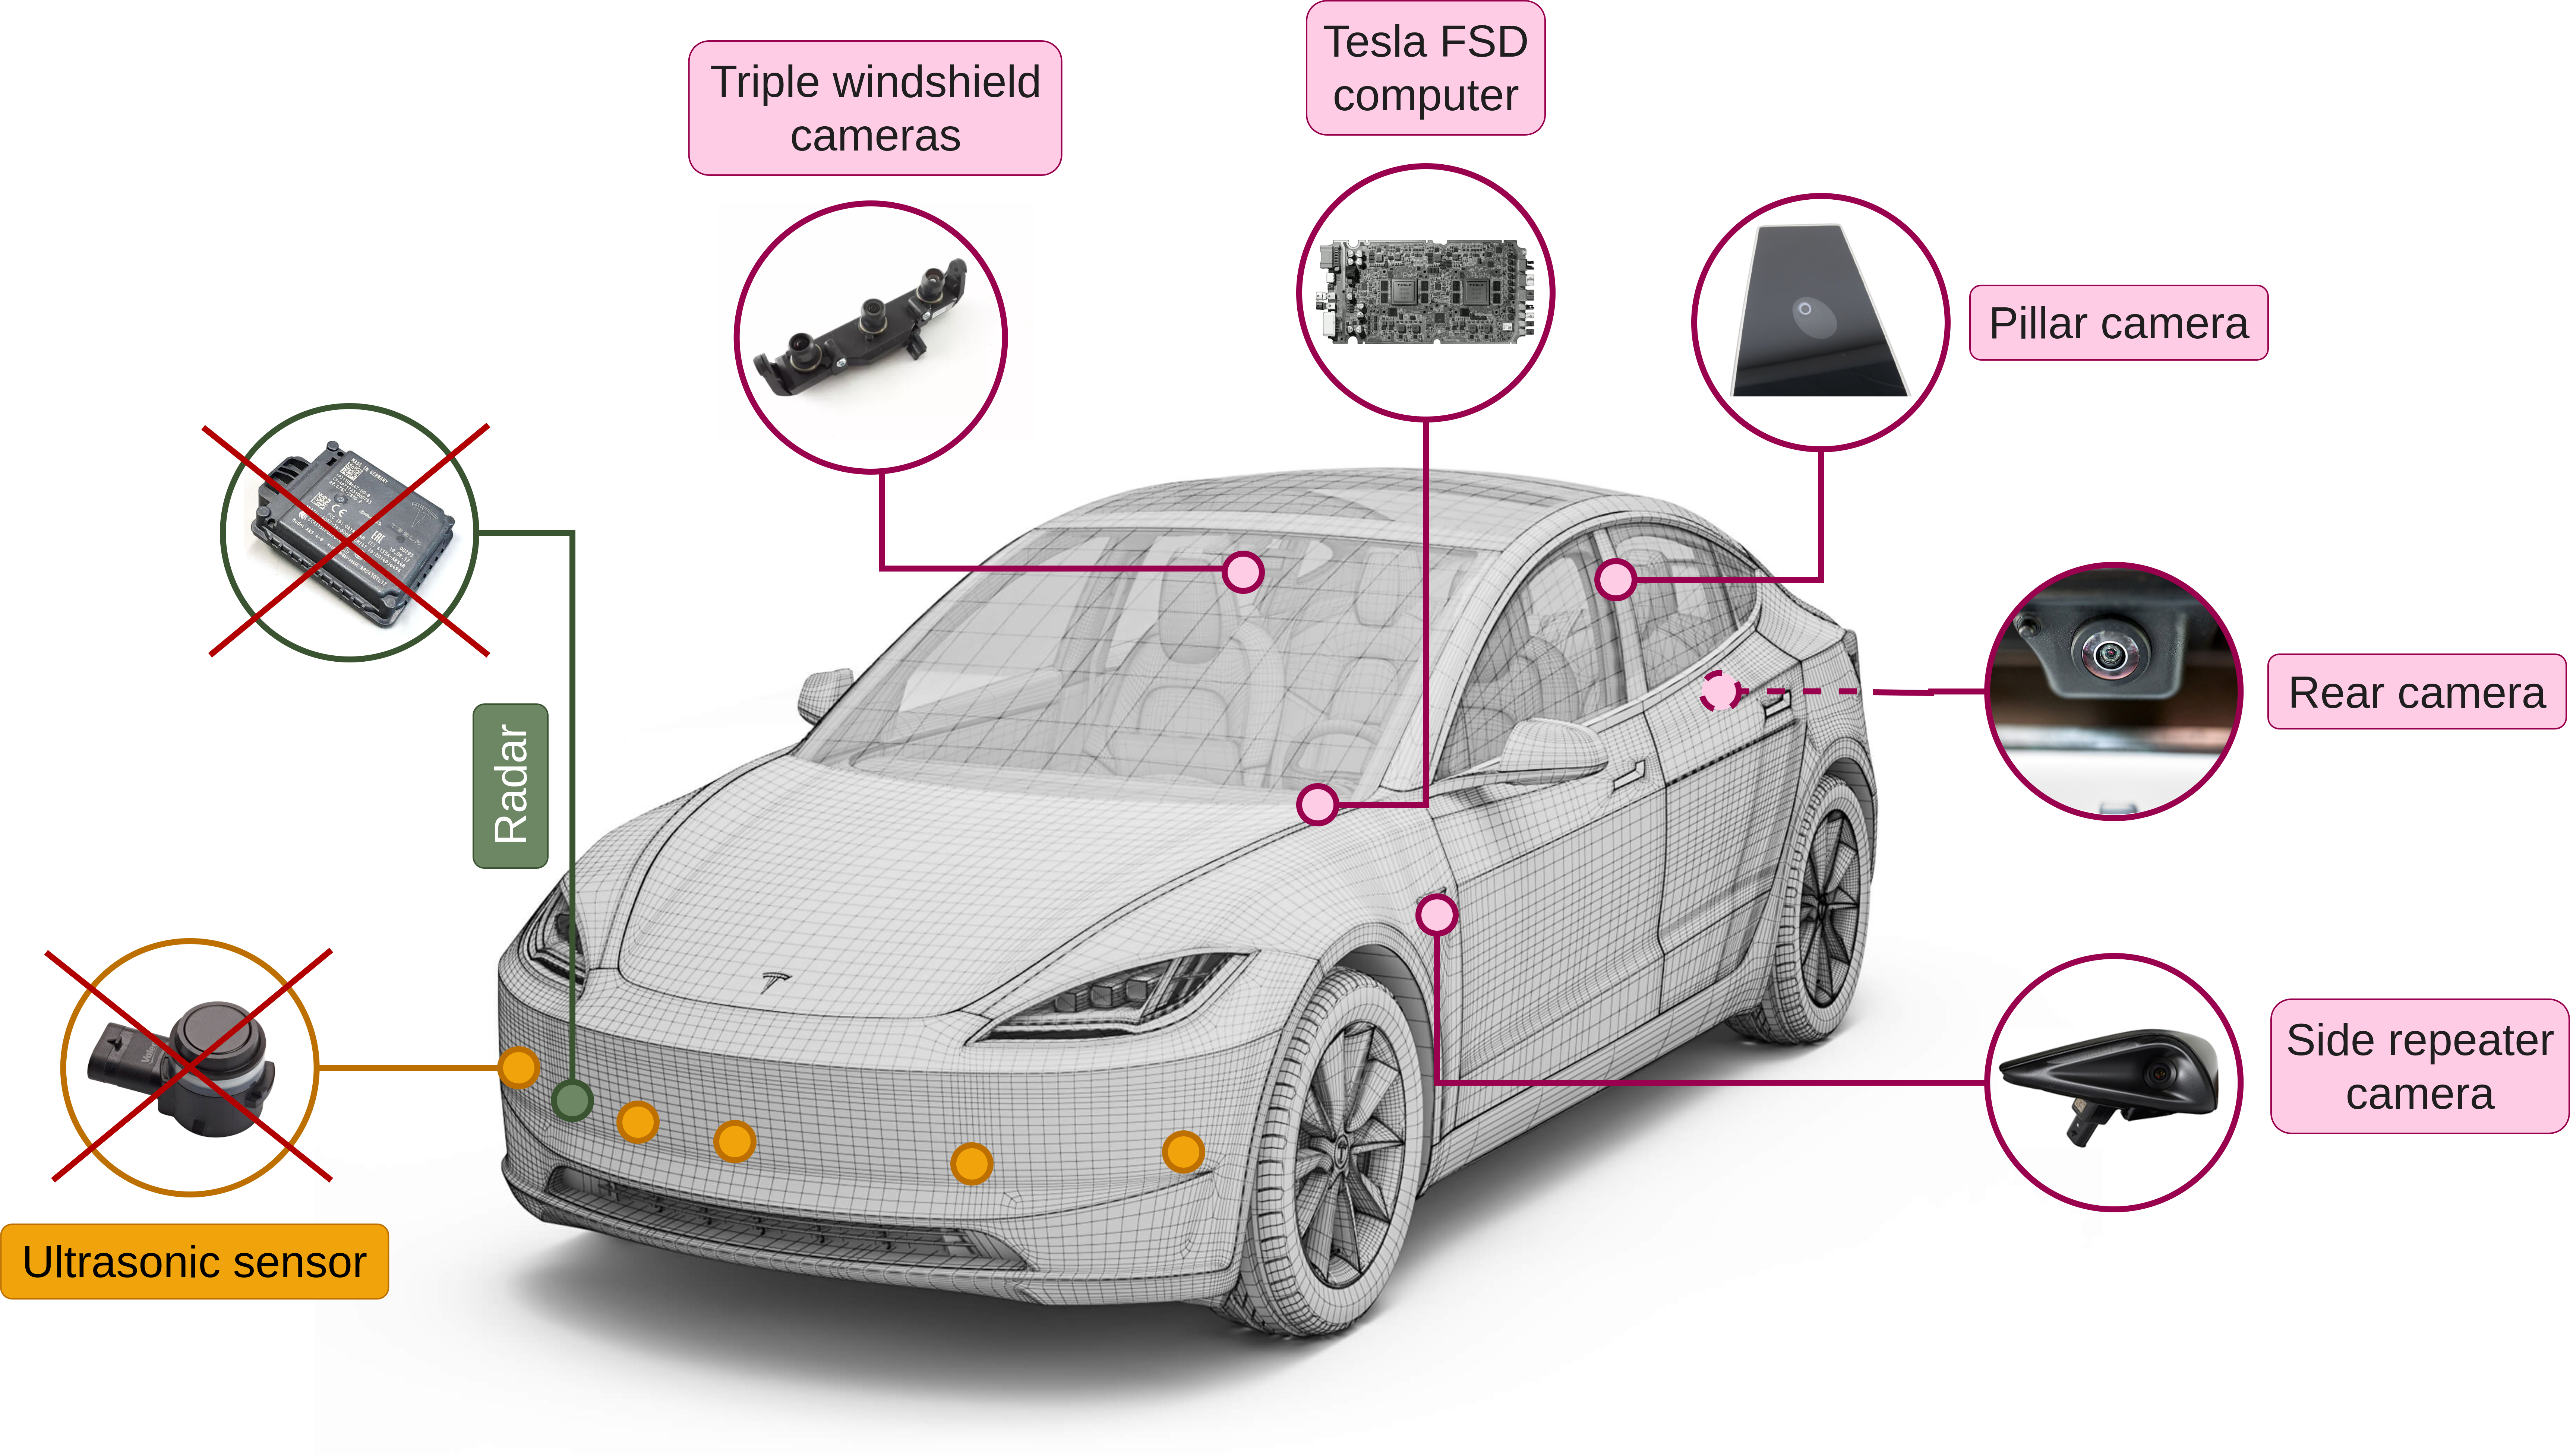
\includegraphics[width=\textwidth]{images/introduction/tesla_sensors.png}
    \caption[Components of an ADAS system]
    {\acs{adas} sensors in a 2024 Tesla Model 3. Modified image source: 
    \cite{mantangcg_2024_tesla_model_3}.}
    \label{fig:adas_components}
\end{figure}

\subsubsection*{Sensors}
Sensors help the vehicle perceive its environment by collecting data on the 
surrounding objects and road conditions. An example of installed sensors on the 
2024 Tesla Model 3 is illustrated in Figure \ref{fig:adas_components}; it is 
possible to notice how also industry is moving towards a fully-computer-vision-based
systems. In fact, Tesla started the transition removing radar sensors in 2021 and 
ultrasonic sensors in 2022, relying only on cameras sensors.
In general, the main types of sensors used in ADAS systems are:

\begin{itemize}
    \item \textbf{Radar Sensors}: These sensors use radio waves to detect the 
    distance and speed of objects around the vehicle. They are particularly 
    useful for measuring the relative speed of other vehicles and detecting 
    objects in poor weather conditions.
    
    \item \textbf{Cameras}: Cameras provide visual data that is used for object 
    recognition, lane detection, traffic sign recognition, and other visual 
    tasks. They are essential for understanding the vehicle's surroundings and 
    identifying potential hazards.
    
    \item \textbf{Ultrasonic Sensors}: These sensors are used for close-range 
    detection, primarily in parking assistance systems. They help the vehicle 
    detect obstacles when maneuvering at low speeds.
    
    \item \textbf{LiDAR}: LiDAR sensors use laser pulses to create a 3D map of 
    the vehicle's surroundings. They are particularly useful for creating 
    detailed maps of the environment and detecting objects at longer ranges.
\end{itemize}

\subsubsection*{Control Units}
Control units are responsible for processing the data from sensors and cameras, 
making real-time decisions, and sending commands to the vehicle's actuators.
Decision making algorithms are implemented in these units to interpret sensor 
data and determine the appropriate response to different driving scenarios.
In the case of Tesla vehicles, the Full Self-Driving (FSD) computer board 
was introduced in 2019, and it is illustrated in Figure \ref{fig:adas_fsd}.
In particular, it is shown the computer board, the chip architecture, and the 
\acf{npu} architecture. The latter is responsible for processing the data 
from the cameras and making real-time decisions based on the input.

\subsubsection*{Actuators}
Actuators are the components that control the vehicle's braking, steering, and 
acceleration systems based on the commands received from the control units. 
These actuators are responsible for executing the decisions made by the ADAS 
to ensure safe and efficient driving.

\subsubsection*{Human-Machine Interface}
The human-machine interface is the system through which the driver interacts 
with the ADAS. This interface includes displays, alerts, and notifications that 
inform the driver about the status of the vehicle and provide warnings or 
assistance when needed. The interface is crucial for ensuring that the driver 
remains aware of the vehicle's behavior and can intervene when necessary.

\subsubsection*{Connectivity}
Connectivity is an essential component of modern ADAS systems, enabling 
communication between the vehicle and external systems. This connectivity allows 
the vehicle to receive real-time traffic information, software updates, and 
remote assistance. It also enables vehicle-to-vehicle and vehicle-to-infrastructure 
communication, which is crucial for advanced safety features like collision 
avoidance and traffic management.

\begin{figure}
    \centering
    
\includegraphics[width=\textwidth]{images/introduction/tesla_fsd.png}
    \caption[Tesla \acs{fsd} computer board and chip architecture]
    {Tesla \acf{fsd} components.
    \textbf{Left}: Tesla \acs{fsd} computer board.
    \textbf{Center}: Tesla \acs{fsd} chip architecture.
    \textbf{Right}: Tesla \acs{fsd} \acf{npu} architecture.
    Modified images sources: 
    \cites{wikichip_2024_tesla_fsd_computer_board}{wikichip_2024_tesla_fsd_chip}{wikichip_2024_tesla_fsd_npu}.}
    \label{fig:adas_fsd}
\end{figure}

\subsection{Common \acs{adas} Features}
ADAS systems offer a wide range of features that enhance vehicle safety, 
comfort, and efficiency. Some of the most common ADAS features include: 
\ac*{acc}, \ac*{ldw}, \ac*{bsd}, \ac*{aeb}, \ac*{tsr}, \ac*{dms}, parking assistance,
adaptive headlights, and more. Most important functionalities are described in detail.

\subsubsection*{\ac{acc}}
\ac{acc} is a feature that maintains a set speed and adjusts it to keep a safe 
distance from the vehicle ahead. It uses sensors to detect the distance and 
speed of the vehicle in front and automatically adjusts the vehicle's speed to
maintain a safe following distance.

\subsubsection*{\ac{ldw}}
\ac{ldw} is a system that alerts the driver if the vehicle begins to drift out 
of its lane without signaling. It uses cameras or sensors to monitor the vehicle's 
position within the lane and provides visual or audible warnings if the vehicle 
starts to veer off course. Some vehicles also have \ac{lka} systems that can 
automatically steer the vehicle back into its lane if the driver does not respond 
to the warnings.

\subsubsection*{\ac{bsd}}
\ac{bsd} is a system that warns the driver of vehicles in the blind spot during
lane changes. It uses sensors to detect vehicles in adjacent lanes that may not
be visible in the side mirrors and provides visual or audible alerts to prevent
collisions during lane changes.

\subsubsection*{\ac{aeb}}
\ac{aeb} is a safety feature that detects imminent collisions with vehicles,
pedestrians, or other obstacles and automatically applies the brakes to prevent
or mitigate the impact. This system helps reduce the severity of accidents by
providing an additional layer of protection when the driver fails to react in
time.

\subsubsection*{\ac{tsr}}
\ac{tsr} is a feature that uses cameras or sensors to identify traffic signs
such as speed limits, stop signs, and road markings. It displays this information
on the vehicle's dashboard or head-up display, helping the driver stay informed
about the current road conditions and regulations.

\subsubsection*{\ac{dms}}
\ac{dms} is a system that monitors the driver's attention and alertness while
driving. It uses sensors to track the driver's eye movements, head position, and
other behavioral cues to detect signs of drowsiness, distraction, or inattention.
The system can provide warnings or take corrective actions to prevent accidents
caused by driver fatigue or distraction.
%
\section{Focus of this work}
\label{sec:focus}
This thesis delves deep into the development of a computer vision-based system 
to warn drivers about potential hazards on the road. The first part is more 
focused on monitoring the driver's behavior and attention through its gaze, and 
outside-world interactions with vulnerable road users. During this phase, 
an initial scheme to analyze the driver's gaze and its interaction with the 
environment is proposed. In particular, the model is based on extracting indirect 
features from sensors, location of vulnerable users during the time, projection 
of the driver's gaze to the scene, and estimation of the depth of the scene.
However, we also highlight the limitations of this approach, mainly due to the 
complexity of the task, and the unreliability of some algorithms used for 
extracting features from the scene.

In the second part, we move to a deep learning-based approach to solve the 
problem of detecting potential hazards on the road. The idea is to have a model 
that can approximate human-like decision making adding some biases to the 
training data.
We focus on training a model 
able to capture the spatial information of the scene, and to predict the presence 
of anomalies in the driving environment. We also explore the possibility of 
leveraging the large quantity of unlabelled data to increase the performance 
of predictions through semi-supervised learning techniques.
At the end, we also explore the potential of few-shots learning with large 
pre-trained models, making some experiments with GPT-4o. This is to demonstrate 
how the model's architecture is suitable for the required tasks with enough 
prior knowledge. It is also interesting to see how the model can adapt to 
the specific domain without changing its parameters and only thanks to the 
attention mechanism.

In the second part we also deeply discuss the training pipeline, which consists 
of data selection and pre-processing, model architecture, and evaluation metrics.
In particular, we analyze how common evaluation metrics can be misleading 
when dealing with unbalanced datasets, and how \ac{roc} and \ac{auc} are 
more reliable metrics for evaluating the performance of the model.
Therefore, we also provide a training method to deal with this type of datasets,
that are prevalent in the field of anomaly detection in driving scenarios.

Another contribution is the discussion of possible future works, 
depending on the results obtained from the experiments and the limitations 
encountered during the development of the project.


\section{Thesis Organization}
\label{sec:organization}
The remainder of this thesis is organized as follows: 
\begin{itemize}
    \item \textbf{Chapter \ref{chpt:related_work}} provides an overview of the 
    state-of-the-art methods and models for object tracking, image and video 
    classification. It discusses how model complexities and relative computational 
    costs increased in the last decade, comparing their performance on benchmark 
    datasets. It also compares available datasets containing driving scenarios 
    for different tasks. Finally, it goes deep into existing model architectures 
    and datasets for anomaly detection in driving scenarios, which is closely 
    connected to our work.
    \item \textbf{Chapter \ref{chpt:background}} presents main algorithms and 
    architectures used for developing the project. It is mainly divided into 
    two sections: traditional computer vision and deep learning-based techniques.
    The former includes explanations of the SIFT algorithm \cite{lowe_sift} and 
    estimation of the homography matrix. The latter includes the Meta Pseudo-Labels 
    algorithm \cite{pham2021meta} and the vision transformer architecture \cite{vit},
    with a focus on all stages involving the multi-head self-attention mechanism.
    \item \textbf{Chapter \ref{chpt:methods}} describes all the methodologies 
    and hypothesis for making the experiments; it is also divided in traditional 
    computer vision and deep learning-based techniques.
    The former includes a general scheme of the driver's attention model, 
    a description of how data is structured and processed, a brief comparison of 
    possible methodologies for estimating the depth, and an explanation of how 
    introducing spatial information of scenes is beneficial.
    The latter includes a general scheme for representing the task to be solved, 
    the training pipeline for making experiments with the DR(eye)VE dataset, and 
    data pre-processing for both DR(eye)VE \cite{dreyeve} and BDD-100K 
    \cite{bdd100k} datasets. 
    \item \textbf{Chapter \ref{chpt:experiments}} shows results obtained from 
    the experiments made with the traditional computer vision and deep learning 
    approaches. For the former case, it includes projection of the gaze, 
    data distribution of the DR(eye)VE dataset, interaction between the 
    driver's gaze and vulnerable road users, accuracy of the monocular depth 
    estimation of MiDaS \cite{midas}, and tracking errors with ByteTrack \cite{bytetrack}. 
    It also discusses limitations of this method 
    and motivations for moving to deep learning-based techniques.
    For the latter case, there are experiments comparing supervised and 
    semi-supervised learning on the DR(eye)VE and BDD-100K dataset. There is also 
    a further experiment on few-shots inference of the GPT-4o model with the 
    BDD-100K dataset, to demonstrate potential performances of task-related 
    knowledge distillation from pre-trained large models to smaller ones
    \cite{yu_knowledge_distillation}.

    \item \textbf{Chapter \ref{chpt:conclusion}} concludes the thesis by summarizing 
    the key contributions, discussing possible problems and limitations that 
    affected the experiments, and outlining potential directions for future work.
    There is also a consideration of how driver's gaze data can be combined with 
    deep learning-based techniques to warn the driver about potential hazards, 
    considering realtime constraints and the need for a reliable system.
    \item \textbf{Appendix \ref{appendix:training_algorithms}} lists main custom 
    algorithms used for the experiments, including data pre-processing and the 
    training pipeline for updating the quantity of labelled samples in the DR(eye)VE dataset.
    \item \textbf{Appendix \ref{appendix:auc_probabilistic}} provides a more 
    formal and detailed explanation of the \acs{auc}-\acs{roc} from a probabilistic
    perspective. It is an helpful appendix to better interpret results on 
    experiments with unbalanced datasets and to understand strenghts and 
    limitations of available evaluation metrics.
\end{itemize}

%
\chapter{Related Work}
We review recent work in behavioral intention prediction through standard 
methods, including object detection and tracking, and more advanced deep learning 
techniques. Moreover, we introduce advantages and limitations of some methods 
that are capable to improve scene understanding.

\section{Available Datasets}
Pedestrian detection and tracking are fundamental tasks in the field of computer 
vision applied to advanced driving assistance systems. If this task is innate 
to humans, it is still a challenging problem for machines. In addition to the 
complexity of the task many applications require real-time processing 
constraints which can affect accuracy of results. 

In the computer vision field object detection can be approached through two f
different perspectives. The former is to make predictions on general datasets 
that are used as benchmarks for the community, such as COCO \cite{coco}.
In this case the goal is to develop a vision model capable to detect a wide 
range of objects, in many different scenarios.
The latter is task-specific oriented, where the goal is to detect a relative 
small subset of objects in a specific context. This is the case of pedestrian 
detection in driving scenarios.

Nowadays, in the field of intelligent transportation systems, many datasets 
have been released to accomplish detection of some common objects, including 
pedestrians, cyclists, and different types of vehicles.
The most common used for benchmarking state of the art algorithms are KITTI 
\cite{kitti}, Berkeley DeepDrive \cite{bdd100k}, Waymo Open Dataset 
\cite{waymo} and nuScenes \cite{nuscenes}. Moreover, each of these datasets 
has its own peculiarity, such as the quantity of video recordings, the variety 
of scenarios, the number of annotated objects, and the quality of ground-truth 
targets, that can be manually annotated or automatically generated.

Despite semi-autonomous driving is getting a lot of attention in the last years 
and it is expected to continue to grow, the state of the art algorithms are far 
away from the robustness and reliability that industry requires. Moreover, it 
has been shown that the performance can drastically drop when models are tested 
on different datasets, and some customized evaluation metrics could be required 
depending on the accomplished task \cite{uricar2019challenges}.
Therefore it is fundamental to deserve as much attention to the quantity and quality of the data 
as to model design process.

\section {Multi-Object Tracking}
Multi-object tracking (MOT) aims to estimate bounding boxes of objects and 
associate them an unique ID across multiple time frames. This task is 
fundamental in perception of the environment because human behaviors are often 
time-dependent. For example it is important to predict pedestrians' trajectories 
to avoid collisions or to understand their intentions. Tracking is performed by 
estimating the future position of objects based on their past spatial and 
temporal information.

Object detection and tracking are distinct tasks, yet both are essential for 
the tracking process. Within tracking, there are two main aims: 
\textit{"tracking by detection"} and \textit{"detection by tracking"}. 
The former leverages powerful modern object detectors to increase tracking 
accuracy. Usually only bounding boxes' features are considered for the task.
The latter, on the other hand, aims to imporve tracking accuracy with the help 
of tracking information. After the detection phase, most MOT methods discard 
some bounding boxes depending on a detection threshold 
\cite{retinatrack,transtrack}; 
therefore all objects related to these boxes are lost for the considered time 
frame. There are also other methods, like ByteTrack \cite{bytetrack}, that are 
able to track partially-occluded objects in real-world scenarios with 
real-time performance. 

For example, ByteTrack does not discard all bounding 
boxes below a certain confidence threshold, but it keeps almost every detection 
dividing them into high score ones and low score ones. At first high score 
detection boxes are matched with corresponding tracklets. Then, due to 
occlusions, resizes and motion blur, remaining unmatched tracklets are 
combined with low score detection boxes. 

\section{Image Classification}
Image classification is a fundamental task in computer vision, as it is also 
used in the detection pipeline. In the last years, many models based on 
convolutional neural networks (CNNs) have been proposed, but nowadays research 
is moving towards more complex classfication tasks using different 
architectures.
The most succesful CNN-based models are, in a chronological order, 
AlexNet \cite{alexnet}, 
VGG \cite{vggnet}, Inception \cite{inception}, ResNet \cite{resnet}, 
DenseNet \cite{densenet} and 
EfficientNet \cite{efficientnet}.

AlexNet \cite{alexnet} was among the pioneering models to incorporate deep convolutional 
layers, stacking five layers that increased the parameter count to 60 million. 
Additionally, it implemented several strategies to mitigate overfitting, 
including the application of dropout. 
Then VGG \cite{vggnet} still increased the number of 
convolutional layers to 16, reaching the state of the art in the ImageNet 
dataset \cite{imagenet}. However, its 138 million parameters made it 
computationally expensive.
Inception \cite{inception}, on the other hand, was able to increase 
the accuracy reducing the model size through multi-scale convolution transforms 
with filters of varying sizes. Transformations were applied to input features 
in parallel, and then concatenated to form the output.
Therefore, it was able to capture diverse spatial information reducing the 
model size to 4 million parameters.
Then ResNet \cite{resnet} brought a revolutional change of CNN architectures, introducing 
the concept of \textit{residual learning}. In particular it addressed the 
problem of vanishing and exploding gradients in very deep models by introducing 
skip connections between layers. This allowed to train a 152-layer CNN model 
that outperformed shallower models.
After ResNet, DenseNet \cite{densenet} introduced another novel aspect by fully connecting 
all convolutional layers with each other in a forward way. 
Unlike traditional CNN architectures where layers are connected in a sequential 
manner, DenseNet establishes direct connections between all layers in a 
feed-forward manner. This dense connectivity enhances feature reuse and 
facilitates gradient flow throughout the network, leading to improved 
parameter efficiency and feature propagation. As a result, DenseNet has shown 
significant improvements in performance and efficiency compared to earlier 
architectures.
Finally, EfficientNet \cite{efficientnet} proposed a new scaling method that uniformly scales 
depth, width, and resolution leading to a better performance. It was able to 
achieve state of the art results on ImageNet as well as on CIFAR-100 while 
being 8.4 times smaller and 6.1 times faster on inference than the best models.

Through this section it was possible to compare main improvements between 
different CNN architectures, and to understand how they evolved over time.
However, by their nature, CNNs are design to extract features from images that 
can be associated to specific object patterns. Through some hyperparameters, 
like kernel size, downsampling, and number of layers, they can be adapted to extract 
features at different scales and with different resolutions. Considering scene 
understanding in driving scenarios, it is fundamental to caputre relative and 
absolute spatial relations of sub-areas in the main scene. 
Therefore, to address this problem, it is necessary to mode towards models 
designed with different architectures, capable to include these kind of 
information. One possible solution is using a vision transformer model (ViT)
\cite{vit}, that is based on the transformer architecture 
\cite{vaswani2023attention}. It consists of a 
self-attention mechanism that allows to tokenize sub-areas of the image and 
capture their spatial relations. This implies that relations are not just 
limited as local features, like with CNNs, but can be extended to all locations 
in the image through the tokens.

In Table \ref{tab:cnn_comparison} a comparison of the discussed models is 
reported. It is possible to see the trending increase of parameters and 
performance over time, but also how since Inception model size has been reduced 
thanks to the introduction of new techniques. It is also possible to notice 
how vision transformer achieves state of the art results with a large model 
size and computational cost, due to the connections between all tokens for 
the self-attention mechanism.

\begin{table}[h]
    \centering
    \begin{tabular}{l|c|c|c|c|c|c}
        \hline
        \textbf{Model} & \textbf{top-1 [\%]} & \textbf{top-5 [\%]} & 
        \textbf{Params.} & \textbf{GFLOPS} & \textbf{Size [MB]} & 
        \textbf{Year} \\
        \hline
        AlexNet & 56.522 & 79.066 & 61.1M & 0.71 & 233.1 & 2012 \\
        \hline
        VGG11 & 69.020 & 88.628 & 132.9M & 7.61 & 506.8 & 2014 \\
        VGG13 & 69.928 & 89.246 & 133.1M & 11.31 & 507.5 & \\
        VGG16 & 71.592 & 90.382 & 138.4M & 15.47 & 527.8 & \\
        VGG19 & 72.376 & 90.876 & 143.7M & 19.63 & 548.1 & \\
        \hline
        Inception\_v3 & 77.294 & 93.45 & 27.2M & 5.71 & 103.9 & 2014 \\
        \hline
        ResNet18 & 69.758 & 89.078 & 11.7M & 1.81 & 44.7 & 2015 \\
        ResNet34 & 73.314 & 91.420 & 21.8M & 3.66 & 83.3 & \\
        ResNet50 & 76.130 & 92.862 & 25.6M & 4.09 & 97.8 & \\
        ResNet101 & 77.374 & 93.546 & 44.6M & 7.8 & 170.5 & \\
        ResNet152 & 78.312 & 94.046 & 60.2M & 11.51 & 230.4 & \\
        \hline
        DenseNet121 & 74.434 & 91.972 & 7.9M & 2.83 & 30.8 & 2016 \\
        DenseNet161 & 77.138 & 93.560 & 28.7M & 7.73 & 110.4 & \\
        DenseNet169 & 75.600 & 92.806 & 14.2M & 3.36 & 54.7 & \\
        DenseNet201 & 76.896 & 93.370 & 20.1M & 4.29 & 77.4 & \\
        \hline
        Effic.Net\_b0 & 77.692 & 93.532 & 5.3M & 0.39 & 20.5 & 2019 \\
        Effic.Net\_b1 & 78.642 & 94.186 & 7.8M & 0.69 & 30.1 & \\
        Effic.Net\_b2 & 80.608 & 95.310 & 9.2M & 1.09 & 35.2 & \\
        Effic.Net\_b3 & 82.008 & 96.054 & 12.3M & 1.83 & 47.2 & \\
        Effic.Net\_b4 & 83.384 & 96.594 & 19.4M & 4.39 & 74.5 & \\
        Effic.Net\_b5 & 83.444 & 96.628 & 30.4M & 10.27 & 116.9 & \\
        Effic.Net\_b6 & 84.008 & 96.916 & 43.1M & 19.07 & 165.4 & \\
        Effic.Net\_b7 & 84.122 & 96.908 & 66.3M & 37.75 & 254.7 & \\
        \hline
        ViT-b\_16 & 81.072 & 95.318 & 86.6M & 17.56 & 330.3 & 2020 \\
        ViT-b\_32 & 75.912 & 92.466 & 88.3M & 4.41 & 336.6 & \\
        ViT-l\_16 & 79.662 & 94.638 & 304.4M & 61.55 & 1161.0 & \\
        ViT-l\_32 & 76.972 & 93.070 & 306.6M & 15.38 & 1169.4 & \\
        ViT-h\_14 & 88.552 & 98.694 & 633.5M & 1016.72 & 2416.6 & \\
        \hline
    \end{tabular}
    \caption{Comparison of the models for image classification on ImageNet}
    \label{tab:cnn_comparison}
\end{table}


\section{Video Classification}
Along with image classification, time-series analysis started gaining attention. 
The initial focus was on univariate and multi-variate input 
data not directly related to images. 
The introduction of Recurrent Neural Networks (RNNs) \cite{rnn} marked a 
significant improvement in analyzing this kind of data. Recurrent neural 
network represents the simplest sequential architecture, and its main 
peculiarity is the presence of a feedback loop that allows to save an internal 
state based on information from previous time steps. Then for each current time 
step the input is combined with the internal state.
Despite the potential of RNNs, they are not able to capture long-term 
information from data sequences. This is due to the vanishing and exploding 
gradient problem, when there are many feedback loops in the network, and it is 
similar to the problem described for deep CNNs.

To address this issue, Long Short-Term Memory (LSTM) \cite{lstm} was introduced. 
LSTM is a modified version of RNN capable to capture both long and short-term 
dependencies in data sequences through specific internal gates. 
A further improvement was introduced with Gated Recurrent Units (GRUs) 
\cite{gru}, that are a simplified version of LSTM with fewer gates and 
parameters.

However, with the advent of image classification in computer vision, 
the interest in video analysis rose. Considering the previous work on RNNs, 
it was natural to extend the concept of time-series analysis to video time 
frames combining RNNs with CNNs. This led to the introduction of 3D CNNs that 
are capable to extract spatio-temporal features from video sequences through 
3D convolutional kernels.

As for image classification, recent developments in the field focused on 
transformer-based models. In particular, the recent ViViT model \cite{vivit} 
utilizes a similar concept of 3D CNNs, but applied to the vision transformer. 
The model stacks images of the video sequence and then applies the transformer 
architecture to capture spatio-temporal relations between them. 
While this approach outperforms 3D CNNs in terms of effectiveness, it comes with 
increased computational costs for training. Additionally, it is required to 
tune numerous hyperparameters.

\section{Semi-Supervised Learning}
Semi-supervised learning (SSL) is a category of machine learning techniques 
that aims to train models using both labeled and unlabeled data. This approach 
is particularly useful when labeled data is scarce and there is a consistent 
amount of unlabeled data available. Large models usually tend to overfit on 
small labeled datasets, and semi-supervised learning can help to mitigate this 
issue by leveraging the information contained in the unlabeled data.
However, to apply semi-supervised learning methods in practice, unlabeled data 
needs to carry useful information that is not already contained in the labeled 
dataset. It has proven to be difficult to find a pratical and sistematic 
approach to address this problem.

To keep the focus on the main topic of this work, we will overview only most 
important self-trianing methods. On the other hand, Engelen et al. 
\cite{ssl_survey} 
provided an up-to-date overview of the field, proposing a complete 
scheme for categorizing semi-supervised learning methods with a complete 
taxonomy.
%
\chapter{Background}
\label{chpt:background}

\section{Meta Pseudo-Labels}
Large models usually tend to overfit on 
small labeled datasets, and semi-supervised learning can help to mitigate this 
issue by leveraging the information contained in the unlabeled data.
However, to apply semi-supervised learning methods in practice, unlabeled data 
needs to carry useful information that is not already contained in the labeled 
dataset. This hypothesis can be formulated through three different assumptions: 
\emph{smoothness}, \emph{clusters}, and \emph{manifold} 
\cite{chapelle2010semi}.

In a more formal formulation, given $p(y|\bm{x}, D_L)$ as the probability 
distribution over the possible classes, given the input $x$ and the labeled 
dataset $D_L$, the goal is to estimate $p(y|\bm{x}, D_L, D_U)$, where $D_U$ is the 
unlabeled dataset. We can say that semi-supervised learning is effective only if 
$p(y|\bm{x}, D_L, D_U)$ is more accurate than $p(y|\bm{x}, D_L)$. If it is not 
the case, semi-supervised learning does not provide any additional benefit to 
the inference of the model, and it could even deteriorate the performance 
\cite{chapelle2010semi}.

\subsection{Smoothness Assumption}
\textbf{Assumption}: If two examples are close in the input space, then they 
have similar outputs (labels).

The smoothness assumption implies that slightly changing the input data should 
not drastically change the output. Therefore, also the model is supposed to 
predict similar outputs for similar inputs. This assumption is fundamental in 
the propagation of the labels on the unlabelled data from the prior knowledge.

In Figure \ref{fig:moon_cluster}, on the left, the smoothness assumption is 
illustrated with an example on the moon dataset. The smoothness assumption 
is satisfied because similar points, in terms of the distance, have the same 
output.

\subsection{Cluster Assumption}
\textbf{Assumption}: Data points are orgnaized in clusters, and points that 
belong to the same cluster are more likely to have the same label.

This assumption supports methods like clustering followed by label propagation, 
where each cluster receives a common label, potentially inferred from a few 
labeled examples within or near the cluster.
It does not imply that each class is related to a unique cluster. 
On the other hand, it means that it is not possible to have two different classes 
in the same cluster.
From this hypothesis, it is also derived the \emph{low-density separation} 
assumption, which imposes that the decision boundary should lie in low-density
regions between clusters.

In Figure \ref{fig:moon_cluster}, on the right, the cluster assumption is 
illustrated with 2D data points organized in clusters. Each cluster's point is 
more likely to have the same label.
\begin{figure}[h]
    \centering
    \begin{minipage}{0.5\textwidth}
        \centering
        \includegraphics[height=5.5cm]{images/ssl/moon.pdf} % first figure
    \end{minipage}\hfill
    \begin{minipage}{0.44\textwidth}
        \centering
        \includegraphics[height=5.5cm]{images/ssl/clusters.pdf} % second figure
    \end{minipage}
    \caption [Illustration of the smoothness and cluster assumptions.]
    {Smoothness and cluster assumptions. \textbf{Left}: The moon dataset representing smoothness between 
        data points of each class. \textbf{Right}: The cluster assumption 
        illustrated with a toy example.}
    \label{fig:moon_cluster}
    \end{figure}
\begin{figure}[h]
    \centering
    \begin{minipage}{0.4\textwidth}
        \centering
        \includegraphics[height=5.5cm]{images/ssl/swiss_roll_3d.pdf} % first figure
    \end{minipage}\hfill
    \begin{minipage}{0.55\textwidth}
        \centering
        \includegraphics[height=5.5cm]{images/ssl/swiss_roll_pca.pdf} % second figure
    \end{minipage}
    \caption[Illustration of the manifold assumption.]
    {Illustration of the manifold assumption. 
        \textbf{Left}: Data points are distributed in a high-dimensional space. 
        \textbf{Right}: The data points lie on a lower-dimensional manifold.}
    \label{fig:swiss_roll}
\end{figure}

\subsection{Manifold Assumption}
\textbf{Assumption}: The data lies on a low-dimensional manifold embedded in a 
high-dimensional space.

This assumption is based on the idea that the data is not distributed uniformly 
in the input space, but it is concentrated on a lower-dimensional manifold.
It is fundamental to avoid problems related to the curse of dimensionality, 
which can lead to overfitting and poor generalization because of sparse data.

In Figure \ref{fig:swiss_roll}, the manifold assumption is illustrated with the 
Swiss roll dataset. The data points are distributed in a three-dimensional 
space, but they lie on a two-dimensional manifold. In general, the principal 
components analysis (PCA) can be used to reduce the dimensionality of the data, 
and in this specific case principal components are respectivlely the $x$ and $z$ 
axes.


\subsection{The Training Algorithm}
Classical pseudo-labeling methods usually train the teacher model on the labeled 
data and then they keep it fixed to predict the labels on the unlabeled data. 
The pseudo-labels are then used to train the student model, which is a copy of 
the teacher model. The student model is finally trained on the pseudo-labelled 
data.

On the other hand, on Meta Pseudo-Labels \cite{pham2021meta}, the teacher is 
trained along with the student model. In particular the student model is trained 
on the pseudo labels generated by the teacher model, and the teacher is trained 
on the performance of the student model on the labeled data. This process is 
repeated until the student model converges reaching a better performance 
with respect to the teacher. Therefore, the teacher model is updated to 
maximize the performance of the student.

In a more formal way, Pseudo Labels aims to optimize the student's 
loss function $CE(T(x_u, \theta_T), S(x_u, \theta_S))$, with the pseudo-labels 
generated from the teacher on the unlabeled data:
\begin{align}
    \theta_S^{PL} &= \arg \min_{\theta_S} \mathbb{E}_{x_u}\left[
        {CE(T(x_u, \theta_T), S(x_u, \theta_S))}\right] 
        \label{eq:pl_student_param}\\
        &:=
        \arg \min_{\theta_S} \mathcal{L}_u(\theta_T, \theta_S) \nonumber
\end{align}

where $T(x_u, \theta_T)$ is the pseudo target generated by the trained teacher 
model with its parameters $\theta_T$ already optimized and fixed. 
Therefore, the final goal of 
Pseudo Labels is to have a lower student loss with respect to the teacher on 
the labelled data:
\begin{align}
    \mathbb{E}_{x_l, y_l}\left[CE(y_l, S(x_l, \theta_S^{PL}))\right]
    &\leq
    \mathbb{E}_{x_l, y_l}\left[CE(y_l, T(x_l, \theta_T))\right]
    \qquad \Longleftrightarrow 
    \label{eq:pl_student_loss}\\
    \mathcal{L}_l(\theta_S^{PL})
    &\leq\
    \mathcal{L}_l(\theta_T) 
    \nonumber
\end{align}

Combining Equations (\ref{eq:pl_student_param}) and (\ref{eq:pl_student_loss}) 
it is possible to notice that the student loss $\mathcal{L}_l(\theta_S^{PL})$ 
depends on the teacher parameters $\theta_T$. Therefore, it could be possible 
get a better optimization of the teacher model to reduce the student loss. 
This is the main idea behind Meta Pseudo-Labels.
The final student loss $\mathcal{L}_l^*(\theta_S^{PL})$ will be the following:
\begin{align}
    \mathcal{L}^*_l(\theta_S^{PL*}) &= \min_{\theta_T} \mathcal{L}_l(\theta_S^{PL}(\theta_T))
    \label{eq:pl_student_loss_final} \\
    \text{where} \qquad \theta_S^{PL}(\theta_T) &= \arg\min_{\theta_S} \mathcal{L}_u(\theta_T, \theta_S)
    \nonumber
\end{align}

However, calculating the gradient $\nabla_{\theta_T}\theta^{PL}_S(\theta_T)$ 
is computationally expensive and complicated to get because it requires to 
unroll all the previous training of the student, given that $\theta_S^{PL}$ was updated 
multiple times with a combination of the fixed $\theta_T$.
To overcome this issue, Meta Pseudo-Labels uses a meta-learning approach to 
approximate  
the computation of $\theta_S^{PL}(\theta_T)$ to a single step:
\begin{align}
    \theta_S^{PL}(\theta_T) &\approx \theta_S - \eta_S \nabla_{\theta_S} \mathcal{L}_u(\theta_T, \theta_S)
    \label{eq:pl_student_update}
\end{align}

where $\eta_S$ is the learning rate used for training the student model.
In this way, the objective function to optimize the student introduced in 
Equation (\ref{eq:pl_student_loss_final}) can be approximated as follows:
\begin{align}
    \mathcal{L}^*_l(\theta_S^{PL}) &\approx \min_{\theta_T} \mathcal{L}_l(\theta_S - \eta_S \nabla_{\theta_S} \mathcal{L}_u(\theta_T, \theta_S))
    \label{eq:pl_student_loss_final_approx}
\end{align}

The final step that distinguishes Meta Pseudo-Labels from other pseudo-labeling 
algorithms is to not keep the teacher fixed during the training of the student. 
With the approximation introduced in Equation (\ref{eq:pl_student_update}), 
the objective function can be updated depending on the information provided only 
at the previous iteration.
Therefore, the teacher is trained along with the student.
The combined training can be summarized in the following steps:

\begin{itemize}
    \item \textbf{Student}: Sample a batch from unlabeled data $x_u$, get the 
    corresponding pseudo-labels $T(x_u, \theta_T)$, and update the parameters: 
    $\theta_S \leftarrow \theta_S - \eta_S \nabla_{\theta_S} \mathcal{L}_u(\theta_T, \theta_S)$.
    \item \textbf{Teacher}: Sample a batch from labeled data $(x_l, y_l)$ and 
    use the new student's parameters to optimize the objective function:
    $\theta_T \leftarrow \theta_T - \eta_T \nabla_{\theta_T} \mathcal{L}_l(\theta_S)$.
\end{itemize}


\section{The Vision Transformer}

Transformers, originally developed for natural language processing tasks, have 
revolutionized the way machines understand and generate text. 
This model architecture, introduced by Vaswani et al. in the paper 
"Attention is All You Need" \cite{attention_is_all_you_need} relies on a 
mechanism known as self-attention to 
process data sequences in parallel, significantly improving efficiency and 
scalability compared to prior methods that used recurrent layers.

Building on the success in NLP, the concept of transformers has been adapted 
for image recognition tasks, marking a significant departure from the 
conventional convolutional neural networks (CNNs) that have dominated the field 
for years. This adaptation was most notably realized in the Vision Transformer 
(ViT) model introduced by Dosovitskiy et al. \cite{vit}. Their research demonstrates how a 
pure transformer applied directly to sequences of image patches can perform at 
or above current state-of-the-art levels on major image recognition benchmarks 
like ImageNet.

This approach challenges the prevailing reliance on CNNs for image tasks, 
suggesting that transformers can equal or exceed CNN performance on benchmarks 
with sufficient training data and computational power. The implications of this 
finding are fundamental, indicating a potential shift towards more flexible and 
scalable models for not only image classification but potentially other computer 
vision tasks as well.
Moreover, it proves that the transformer's ability to handle 
spatial data can be as effective in visual tasks as it has been in 
processing text.

In their paper, "An Image is Worth 16x16 Words: Transformers for 
Image Recognition at Scale" \cite{vit} the authors propose a straightforward yet 
highly 
effective approach: an image is divided into fixed-size patches, these patches 
are linearly embedded, and positional embeddings are added to retain positional 
information. The resulting sequence of vectors is then fed into a standard 
transformer architecture, similar to that used for NLP tasks. The model is 
trained end-to-end for image classification tasks, leveraging extensive 
pre-training on large datasets followed by fine-tuning on targeted smaller 
datasets.

\begin{figure}
    \centering
    \includegraphics[width=0.8\textwidth]{images/vit/vit_scheme.png}
    \vspace*{0.3cm}
    \caption[The Vision Transformer architecture.]
    {The Vision Transformer architecture \cite{vit}. The input image is divided 
    into fixed-size patches, linearly embedded, and positional embeddings are 
    added. The resulting sequence of vectors is fed into the transformer encoder 
    architecture. On the top a feed-forward layer performs the classification.}
    \label{fig:vit_architecture}
\end{figure}

\subsection{Patch Embeddings}
Patch embedding is a key process that transforms raw image data into a format 
suitable for the transformer architecture. An image is first divided into small 
patches, which can be considered as sub-areas of the input image. 

Each patch is then flattened and projected into a higher-dimensional space 
through a linear transformation. This creates dense vector representations of 
the patches, like the word embedding process in NLP. 
Positional embeddings are added to these patch embeddings to preserve their 
spatial relationships, allowing the transformer to understand the layout of the 
image as it processes the sequence of embedded patches. 

This method adapts the transformer's powerful self-attention mechanisms to 
handle and interpret spatial relations of visual data.


\subsection{Self-Attention Mechanism}
The core of the transformer architecture is the self-attention mechanism, which 
allows the model to weigh the importance of different parts of the input data.
It is worth noting that the fundamental concept of self-attention does not 
require any trainable parameters. It is actually computed only through the 
embedded patches.

Considering a sequence of embedded patches $\{\boldsymbol{x_1, x_2, ..., x_t}\}$ 
as input, the self-attention is a sequence-to-sequence operation that outputs
$\{\boldsymbol{y_1, y_2, ..., y_t}\}$. The goal is to have each output vector 
$\boldsymbol{y_i}$ that represents a similarity between the $i$-th 
patch and all the input sequence of patches. In particular it can be described by a  
weighted sum of the input sequence
\begin{equation}
\boldsymbol{y_i} = \sum_{j=1}^{t} w_{ij} \boldsymbol{x_j}
\label{eq:self_attention_output}
\end{equation}
where $\boldsymbol{w_i}:=\{w_{ij}\}_{j=1}^t$ is the set of weights that describes the importance 
of each input vector for the $i$-th one. 
Therefore each $i$-th vector has a different set of weights with respect to 
the others.

The simplest way to compute the similarity is to use the dot-product between the 
input vectors $w'_{ij} = \boldsymbol{x_i^T x_j}$. Moreover, to guarantee them to have a limited 
range in $(0, 1)$ and to sum up to $1$, the softmax function is applied:
\begin{equation}
    w_{ij} = \boldsymbol{\sigma}(\boldsymbol{w'_i})_j = 
    \frac{e^{w_{ij}}}{\sum_{j} e^{w_{ij}}}
    \label{eq:attention_weights}
\end{equation}
From Equation (\ref{eq:attention_weights}) it is possible to notice that the 
weights depend only on the input vectors, and they are computed independently. 
That means that the self-attention mechanism is a parallel operation that does 
not consider the order of the input sequence. If the input sequence order is 
changed then the output sequence will change the order as well, keeping the 
same similarity results.

\subsection{Queries, Keys and Values}
In the self-attention task, each input vector $\boldsymbol{x_i}$ plays three 
different roles:
\begin{itemize}
    \item \textbf{Query}: $\boldsymbol{x_i}$ is used to compute the similarity to all the other 
    vectors in order to calculate $y_i$.
    \item \textbf{Key}: $\boldsymbol{x_i}$ is used to compute the similarity of 
    all the other vectors with respect to itself, in order to calculate all the 
    other outputs.
    \item \textbf{Value}: $\boldsymbol{x_i}$ is used to compute the weighted sum 
    of the input vectors, given the weights already computed.
\end{itemize}
This method introduces some controllable parameters that can be learned during 
the training to accomplish the respective tasks. In particular, the matrices 
are $\boldsymbol{W_q}, \boldsymbol{W_k}, \boldsymbol{W_v}$ and they all have 
dimesion $(q_k, q_k)$, given $q_k$ the embedding dimension of patches.
Equations (\ref{eq:self_attention_output}) and (\ref{eq:attention_weights}) can 
be rewritten as follows:
\begin{equation}
\begin{cases}
    w_{ij} = \boldsymbol{\sigma}(\boldsymbol{K^T q_i})_j \\
    \boldsymbol{y_i} = \sum_j w_{ij} \boldsymbol{v_j}
\end{cases}
\qquad
\text{where}
\quad
\begin{cases}
    \boldsymbol{q_i} = \boldsymbol{W_q x_i} \\
    \boldsymbol{K} = \boldsymbol{W_k X} \\
    \boldsymbol{v_j} = \boldsymbol{W_v x_j} \\
    \boldsymbol{X} = (\boldsymbol{x_1}, ..., \boldsymbol{x_t})
\end{cases}
\label{eq:self_attention_qkv}
\end{equation}
It is worthwile ntoicing that it is easier to consider the queries and values 
vectors, and the keys matrix. That is because the query is referred a specific 
input vector that is used to compute the similarity with all the others. 
The value is still directly related to the input vector used to compute the 
weighted sum. On the other hand, the keys are related to all the input vectors. 
Therefore, multiplying a query with the keys matrix will give all the similarities 
for the selected vector.

Adding trainable parameters to the self-attention mechanism allows to figure out 
the importance of all the sub-areas of the input image, depending on the bias we 
use to label the dataset. Then it is possible to use the attention mask, to 
highlight the importance of some specific areas of the image.

Finally, dot products between rows of $\boldsymbol{K^T}$ and 
$\boldsymbol{q_i}$ typically grow with the dimension of the embedding, 
and it can lead to instabilities in terms of gradients during the learning 
process. Therefore it is common to normalize the dot product by the square root 
of the embedding dimension $\sqrt{d_k}$, considering that it is also the 
grow rate of the Euclidean distance of the input vectors.

In a more general matrix form, Equation (\ref{eq:self_attention_qkv}) with the 
normalization can be 
described as follows:
\begin{equation}
Y = \boldsymbol{\sigma}\left(\boldsymbol{\frac{K^T Q}{\sqrt{d_k}}}\right) V\\
\qquad
\text{where}
\quad
\begin{cases}
    \boldsymbol{Q} = \boldsymbol{W_q X} \\
    \boldsymbol{K} = \boldsymbol{W_k X} \\
    \boldsymbol{V} = \boldsymbol{W_v X} \\
    \boldsymbol{X} = (\boldsymbol{x_1}, ..., \boldsymbol{x_t})
\end{cases}
\label{eq:self_attention_qkv_matrix}
\end{equation}
In Equation (\ref{eq:self_attention_qkv_matrix}) the softmax function 
$\boldsymbol{\sigma}$ is applied to the rows of its argument.


\subsection{Multi-Head Self-Attention Mechanism}
In an image each patch can have different relations with the others, depending 
on the context. Therefore, using only one self-attention mechanism would sum all 
the information together, limiting the ability to capture the scene context. 
To overcome this issue, the multi-head self-attention mechanism is introduced.
It is a parallel operation based on the single self-attention mechanism, which 
introduces multiple weight matrices $\boldsymbol{W_q^r, W_k^r, W_v^r}$, also 
called \emph{attention heads}.

It is also possible to keep the same number of parameters of the single 
self-attention mechanism in an efficient way. The main idea is to project queries, 
keys and values to a lower-dimensional space according to the number of heads.
In particular, given $h$ the number of attention heads, $d_k$ the embedding 
dimension of the patches, we can use a transformation matrix 
$\boldsymbol{T^r}$ of dimension $\left(d_k, d_k/h\right)$.
Therefore, the total number of parameters for
the single-head and multi-head self-attentions will be:
\begin{align*}
    \text{\#params SHA} &= 3 \cdot d_k^2 \\
    \text{\#params MHA} &= 3 \cdot h \cdot d_k \cdot\frac{d_k}{h} = 3 \cdot d_k^2
\end{align*}
\begin{figure}[htbp]
    \centering
    \includegraphics[width=\textwidth]{images/vit/multi_head_attention_scheme.png}
    \caption[Multi-head self-attention mechanism.]
    {Multi-head self-attention mechanism schematically represented with 
    the main blocks: patch embeddings, dimension reduction, attention heads, 
    data concatenation, and final linear transformation.}
    \label{fig:multi_head_attention}
\end{figure}
In Figure \ref{fig:multi_head_attention} the multi-head self-attention mechanism 
is schematically represented, and data flow is from the bottom to the top. 
The input patches are first embedded and projected to a lower-dimensional space. 
Therefore we get queries, keys and values for each attention head. 
The self-attention mechanism is applied to each head, and the outputs are 
concatenated together. In this way we augment the information of the spatial 
relation of each patch. Finally, a linear transformation is applied to get 
the final output of the multi-head self-attention mechanism, which describe the 
attention of each patch with respect to all the others.

To avoid any misunderstanding on the generation of the queries, keys, values and 
on the concatenation, data is represented through channels, where each channel is 
related to a specific attention head and it is independent from the others.

It is also worth noticing that the transformer architecture leverages on residual 
connections and layer normalization to stabilize the training process, avoiding 
the vanishing gradient problem. The residual connections are used to sum the 
output of the multi-head self-attention mechanism with the embedded patches, 
and the layer normalization is applied to the sum.

\subsection{Classification Transformer}
If the final task is a classification of the input image, it is necessary 
to have a feed-forward layer on the top of the transformer encoder, as shown in 
Figure \ref{fig:vit_architecture}.
Therefore, the final output will depend on the relative relation of the patches 
and their absolute location in the image.


\section{Traditional Computer Vision Techniques}
In this section we refer to some methods that have been used for a long time 
in computer vision tasks, even before the deep learning era. These methods 
are still used in some specific tasks, usually related to multiple view geometry.
In particular, the following methods are described: the \ac{sift} \cite{lowe_sift}, 
the Random Sample Consensus (RANSAC) \cite{ransac}, and the optimization 
algorithm to estimate the homography between two images.

\subsection{Scale Invariant Feature Transform (SIFT)}
The \ac{sift} algorithm is a method to detect and describe local features in 
images. It was introduced by David Lowe in 2004 \cite{lowe_sift}, and it is 
still used in computer vision tasks thanks to its robustness to changes in 
illumination, rotation, and scale. However, being computationally expensive, 
it is difficult to integrate it in real-time applications. Therefore other 
versions of the algorithm have been developed, like \ac{surf} \cite{surf} and
\ac{asift} \cite{asift}. These algorithms have also been implemented in 
computer vision libraries, like OpenCV, to leverage the power of parallel 
computing of GPUs.

The \ac{sift} algorithm is based on the following steps: scale-space peak
selection, keypoints detection, and assignment of descriptors to the keypoints.

\subsubsection{Scale-Space Peak Selection}
To make the algorithm robust and scale-invariant, the first step is to analyze 
the image at different scales, applying a Gaussian filter with different 
standard deviations. Given an image $I(x, y)$, the scale-space representation 
is defined as: 
\begin{equation}
    L(x, y, \sigma) = G(x, y, \sigma) * I(x, y)
    \label{eq:scale_space}
\end{equation}
where $G(x, y, \sigma)$ is the Gaussian kernel with standard deviation $\sigma$.
The scale-space representation is computed for different values of $\sigma$, and 
the process is repeated for different octaves of the image. An octave is 
a set of images, each one with a resolution half of the previous one. The number 
of images for each octave is not standard, and it depends on the resolution 
of the original image.

The scale-space representation is used to detect the local maxima and minima 
of the difference of Gaussian (DoG) function. The DoG function is computed as 
the difference between two consecutive images of the same octave (let's say 
they have standard deviations $\sigma$ and $k\sigma$):
\begin{equation}
    D(x, y, \sigma) = L(x, y, k\sigma) - L(x, y, \sigma)
    \label{eq:dog}
\end{equation}
The local maxima and minima of the DoG function are detected by comparing each 
pixel with its eight neighbors in the same image and the nine neighbors in the 
previous and next images (26 in total). If the pixel is a local maxima or minima, it is 
considered a keypoint. To be a maxima or minima, the candidate pixel must be 
greater or smaller than all the neighbors, respectively.

\subsubsection{Keypoints Localization}
The scale-space peak selection produces many keypoints, but not all of them are 
stable under changes in illumination, rotation, and scale. Therefore, the 
keypoints are filtered by applying the Taylor expansion to the DoG function 
for each candidate keypoint. The Taylor expansion is used to estimate 
the actual maxima or minima of the DoG function, approximated by the 
second-order derivative of the function with respect to the selected keypoint.

Considering the DoG function $D$ related to a keypoint, and an offset 
along all the dimensions
$\boldsymbol{x} = (dx, dy, d\sigma)^T$, 
to find accurate location of the selected keypoint a second-order Taylor expansion 
is computed as follows:
\begin{equation}
    D(\boldsymbol{x}) = D + \frac{\partial D}{\partial \boldsymbol{x}}^T \boldsymbol{x} + 
    \frac{1}{2} \boldsymbol{x}^T \frac{\partial^2 D}{\partial \boldsymbol{x}^2} \boldsymbol{x}
    \label{eq:taylor_expansion}
\end{equation}
Minima, or maxima, $\boldsymbol{\hat{x}}$ is detected by solving the equation:
\begin{equation}
    \boldsymbol{\hat{x}} = \arg \min_{\boldsymbol{x}} D(\boldsymbol{x})
    = \arg \{ \nabla_{\boldsymbol{x}} D(\boldsymbol{x}) = \boldsymbol{0} \}
\end{equation}

Keypoints with low intensity are filtered out, depending on a threshold. Therefore, 
the more accurate keypoint $\boldsymbol{\hat{x}}$ is discarded if:
\begin{equation}
    D(\boldsymbol{\hat{x}}) < \text{threshold}
\label{eq:contrast_threshold}
\end{equation}

To remove the keypoints that are located on edges, on the other hand, the ratio 
between the principal curvatures of the DoG function is computed. 
If the ration is greater than a threshold, it means that there is a high variation 
of intensity on one direction with respect to the other (typical of an edge). 
Otherwise the keypoint corresponds to a corner and it is kept.
Principal curvatures are given by the eigenvalues $\lambda_1$ and $\lambda_2$
of the Hessian matrix of the 
DoG function, and the ratio is computed as follows:

\begin{equation}
    \frac{\text{Tr}(H)^2}{\text{Det}(H)} = \frac{(r+1)^2}{r} < \text{threshold}
    \qquad
    \text{where:} \quad r = \frac{\lambda_1}{\lambda_2}
    \label{eq:edge_threshold}
\end{equation}
It is possible to notice that the evaluation function in Equation 
(\ref{eq:edge_threshold}) has a minimum when the two eigenvalues are equal, 
and it grows when the ratio between the two eigenvalues increases.

\subsubsection{Keypoint Orientation}
To make the keypoints invariant to rotation of the image, the orientation with 
respect to the neighbor pixels is computed. The orientation is computed through 
two terms, the magnitude and the orientation of the gradient of the 
correspondent DoG function:
\begin{align*}
    m(x, y) &= \sqrt{\left[D(x+1, y) - D(x-1, y)\right]^2 + \left[D(x, y+1) - D(x, y-1)\right]^2} \\
    \theta(x, y) &= \arctan\left(\frac{D(x, y+1) - D(x, y-1)}{D(x+1, y) - D(x-1, y)}\right)
\end{align*}
The angle $\theta$ is computed in the range $[0, 2\pi]$, and it is quantized 
in a histogram with 36 bins. The assigned orientation consists of the peak of 
the histogram, and all the other peaks that are greater than 80\% of the maximum.

\subsubsection{Keypoint Descriptor}
After having assigned the orientation to the keypoints, the final step is to 
assign a unique descriptor to each keypoint. 
A grid of 16x16 pixels is considered around the keypoint, and it goruped into 
4x4 macro-areas. For each macro-area, the gradient magnitude and orientation 
are computed, and they are grouped into 8 bins. Therefore, the descriptor is 
a 128-dimensional vector (4x4x8).

To make the descriptor invariant to rotation, the orientation of the keypoint 
is subtracted from each gradient orientation.
Moreover, to make the descriptor invariant to illumination changes, each 
magnitude is truncated to a maximum thrashold, and then normalized.

\subsubsection{Matching Keypoints}
To match similar keypoints in two different images, the Euclidean distance 
between the descriptors can be computed. However, considering a descriptor, 
there could be more than one similar match on the other image (i.e. the second 
best match could be close to the best). To overcome this issue, the ratio between 
the best and the second best match is computed. If the ratio is less than a 
threshold, the match is considered valid.

\subsection{Projective Transformation}
A homography is the transformation between two planes under perspective projection.
This means that a planar object in transformed by a homogeraphy into its image 
sensor.
However, the transformation can also be seen between two cameras, if all points 
in the Euclidean space lie on the same plane.

In Figure \ref{fig:homography_scheme} the homography transformation between two 
camera planes is represented. Two cameras, with their own system of coordinates, 
are pointing to the same plane. All points in the Euclidean space lie on the 
same plane, and they are projected on the two cameras' planes. The homography 
matrix $\boldsymbol{H}$ is the transformation of the projected points between 
the two camera planes.

Considering a general point $P_i \in \mathbb{R}^{3}$ in the Euclidean space, 
lying on a plane, and its correspondent projections on the two cameras' planes
$\boldsymbol{p_i}, \boldsymbol{p_i'} \in \mathbb{R}^{2}$.
Without focusing on a specific point, and without loss of generality, projection 
can be described by the following equation:
\begin{align}
    \boldsymbol{\tilde{p}} &\sim \boldsymbol{H} \boldsymbol{\tilde{p}'} && \boldsymbol{H} \in \mathbb{R}^{3 \times 3}, 
    \label{eq:homography}\\
    & && \boldsymbol{\tilde{p}}, \boldsymbol{\tilde{p}'} \in \mathbb{P}^{2}\nonumber
\end{align}
where $\boldsymbol{\tilde{p}}$ and $\boldsymbol{\tilde{p}'}$ are homogeneous 
coordinates of the points $\boldsymbol{p}$ and $\boldsymbol{p'}$ in the 2D
projective space $\mathbb{P}^{2}$. It is worth to notice that $\boldsymbol{H}$ 
is the homography matrix, and it is defined up to a scale factor. Therefore, to 
fully define it, at least four correspondent points are required.
Considering homogeneous coordinates of the points, Equation (\ref{eq:homography}) 
can be rewritten as follows:
\begin{equation}
    \begin{bmatrix}
        x \\
        y \\
        1
    \end{bmatrix}
    =
    \begin{bmatrix}
        h_{11} & h_{12} & h_{13} \\
        h_{21} & h_{22} & h_{23} \\
        h_{31} & h_{32} & h_{33} \\
    \end{bmatrix}
    \begin{bmatrix}
        x' \\
        y' \\
        1
    \end{bmatrix}
    \label{eq:homography_matrix}
\end{equation}
\begin{figure}
    \centering
    \includegraphics[width=0.6\textwidth]{images/dreyeve/homography.png}
    \vspace{0.2cm}
    \caption[Homography scheme.]
    {Homography between two planes. The transformation matrix defines the 
    projection between the camera planes. All points in the Euclidean space 
    lie on the same plane.}
    \label{fig:homography_scheme}
\end{figure}

\subsubsection{Homography Estimation}
Given the $i$-th correspondance between two images, defined by the set 
$\{(x_i, y_i), (x_i', y_i')\}$, constraints described in Equation \ref{eq:homography_matrix}
are:
\begin{align}
&\begin{cases}
    x_i' = h_{11} x_i + h_{12} y_i + h_{13} \\
    y_i' = h_{21} x_i + h_{22} y_i + h_{23} \\
    1 = h_{31} x_i + h_{32} y_i + h_{33}
\end{cases}
\qquad \Longleftrightarrow \nonumber\\[0.2cm]
&\begin{cases}
    x_i' \left(h_{31} x_i + h_{32} y_i + h_{33}\right) = h_{11} x_i + h_{12} y_i + h_{13} \\
    y_i' \left(h_{31} x_i + h_{32} y_i + h_{33}\right) = h_{21} x_i + h_{22} y_i + h_{23}
    \label{eq:homography_constraints}
\end{cases}
\end{align}
In a matrix form, rearranging the terms to explicit terms of the homography matrix,
Equation (\ref{eq:homography_constraints}) can be written as:
\begin{equation}
    \begin{bmatrix}
        x_i & y_i & 1 & 0 & 0 & 0 & -x_i'x_i & -x_i'y_i \\
        0 & 0 & 0 & x_i & y_i & 1 & -y_i'x_i & -y_i'y_i
    \end{bmatrix}
    \begin{bmatrix}
        h_{11} \\
        \vdots \\
        h_{33}
    \end{bmatrix}
    =
    \begin{bmatrix}
        x_i' \\
        y_i'
    \end{bmatrix}
    \label{eq:homography_matrix_constraints}
\end{equation}
Considering now a general case with $n$ correspondences the problem to solve 
becomes in the form:
\begin{equation}
\begin{bmatrix}
    x_1 & y_1 & 1 & 0 & 0 & 0 & -x_1'x_1 & -x_1'y_1 & -x_1'\\
    0 & 0 & 0 & x_1 & y_1 & 1 & -y_1'x_1 & -y_1'y_1 & -y_1'\\
    \vdots & \vdots & \vdots & \vdots & \vdots & \vdots & \vdots & \vdots & \vdots \\
    x_n & y_n & 1 & 0 & 0 & 0 & -x_n'x_n & -x_n'y_n & -x_n'\\
    0 & 0 & 0 & x_n & y_n & 1 & -y_n'x_n & -y_n'y_n & -y_n'
\end{bmatrix}
\begin{bmatrix}
    h_{11} \\
    \vdots \\
    h_{33}
\end{bmatrix}
=
\boldsymbol{0}
\label{eq:homography_matrix_constraints_general}
\end{equation}
Equation (\ref{eq:homography_matrix_constraints_general}) is in the form of 
$\boldsymbol{Ah} = \boldsymbol{0}$, where $\boldsymbol{A} \in \mathbb{R}^{3x3}$
and $\boldsymbol{h} \in \mathbb{R}^{9}$.
When the number of correspondences is greater than 4, the system is overdetermined, 
and the homography matrix can be estimated by solving the least squares problem:
\begin{equation}
    \boldsymbol{h}^* = \arg \min_{\boldsymbol{h}} \left\| \boldsymbol{Ah} \right\|
    \quad
    \text{such that }
    \left\| \boldsymbol{h} \right\| = 1
    \label{eq:homography_least_squares}
\end{equation}

%
\chapter{Methods}

\section{Classical Computer Vision-based Approach}

This section is related to all the experiments done on the classical computer 
vision-based approach. The general scheme of the driver's attention model is 
shown in Figure \ref{fig:driver_attention}. 
The model is divided into four main stages: data synchronization, homography 
projection of the gaze, scene perception, and the driver's behavioral model. 

The data synchronization stage is responsible for aligning the data from the 
different sensors. In particular it is important that gaze data and 
images from the 
eye-tracking glasses are well synchronized each other and with video frames 
from the camera installed on the roof top of the car.

The homography projection of the gaze stage is responsible for projecting the 
gaze of the driver from the ETG camera plane to the roof top camera plane.
In this way we have a wider, more stable and accurate representation of 
the outside environment.
It is possible to 
estimate the homography transformation making the approximation that the matched 
keypoints are far away enough from the vehicle. This is a reasonable 
approximation since the driver is usually looking at the road and the objects 
far away from the vehicle. Moreover, the baseline of the stereo vision system is 
small compared to the depth of the keypoints.
The optimal way to estimate the projection would be through the epipolar 
geometry, estimating the fundamental matrix and the essential matrix. 
However, we have an uncalibrated stereo setup, and the baseline between the two 
cameras is not fixed. Even though it could be possible to integrate GPS data 
to estimate the two matrices, there is a consistent noise error that affects 
accuracy of the estimation.
The homography estimation is then divided in three steps: detection of keypoints 
in the two images through the SIFT algorithm, matching of the keypoints through 
RANSAC, and estimation of the homography matrix through the least squares method.

The scene perception stage is responsible for detecting and tracking the vulnerable 
users in the scene, such as pedestrians and cyclists. The detection is done 
through the YOLOv8 algorithm and the tracking through ByteTrack. In this way 
it is possible to compare the gaze of the driver with the state of the targets, 
including their position.

Finally, on the top, there is the driver's attention model. The responsibility 
of this block is to classify dangerous scenarios given the data from the 
driver and the scene. However, this block is sensitive to the quality of the 
signals of the previous stages.

\begin{figure}
    \centering
    \includegraphics[width=0.9\textwidth]{images/dreyeve/classic_scheme.png}
    \vspace*{0.6cm}
    \caption{The overall driver's attention scheme. It is divided into four main 
    stages: data synchronization, homography projection of the gaze, scene 
    perception and the driver's behavioral model.
    }
    \label{fig:driver_attention}
\end{figure}

\subsection{Homography Data Structure}
The Dr(eye)ve dataset is composed of 74 sequences of five minutes each. 
Moreover, the two cameras are not synchronized. 
The ETG camera has a frame rate of 30 fps, while the roof top camera has a 
frame rate of 25 fps. It is also important to notice that there are some videos 
that was recorded at slightly different frame rates. All the synchronization data 
are provided in the dataset.

Therefore, we decided to implement 
an interface to preprocess all the frames and synchronize them.
After the synchronization, we compute all the homographies and store them in a 
file. This file is then used to project the gaze of the driver in the roof top 
camera plane.
Furthermore, we chose to store other informations related to the quality of the 
estimation.
The data structure is described in Figure \ref{fig:homography_data_structure}:
it is a list of lists where each element is a unique sample that has the 
following fields: the gaze coordinates in the ETG and RT camera planes, the 
homography matrix, detected keypoints on the two planes, and the number of 
matchings between them.

\begin{figure}
    \centering
    \includegraphics[width=\textwidth]{images/dreyeve/homography_data.png}
    \caption{The data structure used to store the homographies.
    \textbf{Left}: Each element is a specific sample in the i-th video, at 
    the j-th frame.
    \textbf{Right}: The attributes of each sample.}
    \label{fig:homography_data_structure}
\end{figure}

\subsection{Stereo Camera System Setup}
The cameras recording system can be reconducted to an uncalibrated stereo vision 
setup. In particular, the two cameras are not aligned and the baseline is not 
fixed. However, this is a problem for the projection of 3D world points between 
the two cameras. In fact, homography is a planar transformation, 
and it is possible to estimate the projection matrix if keypoints lie on the 
same plane.
For this reason we decided to make the approximation that the 
keypoints are far away enough from the vehicle. This is a reasonable 
approximation since the driver is usually looking at the road and the objects 
far away from the vehicle. Moreover, the baseline of the stereo vision system is 
small compared to the average depth of the keypoints.

In this way, it is not necessary to know intrinsic and extrinsic parameters of 
the cameras, such as focal length, resolution, and distortion coefficients. 
This approach is also proposed in the Dr(eye)ve paper \cite{dreyeve}.


\subsection{Targets Data Structure}
From the Dr(eye)ve dataset, we extracted the bounding boxes of the vulnerable 
road users, such as pedestrians and cyclists.
Moreover, through ByteTrack \cite{bytetrack}, we tracked the targets to have a 
spatio-temporal representation of the scene. Then, we compare the projected gaze 
of the driver with the location of targets. 

However, it is necessary to consider the quality of the tracking. Even though 
ByteTrack was specifically designed to track also overlapping objects, in driving 
scenarios it is not uncommon to have tracking failures. To partially mitigate 
the problem, we set two different states for each target: a 
\emph{detection} state and an \emph{observation} state.
\begin{itemize}
    \addtolength\itemsep{-2mm}
    \item \textbf{Detection}: the target is being detected and tracked by the algorithms.
    \item \textbf{Observation}: the target is being observed by the driver.
\end{itemize}

\begin{figure}
\centering
\includegraphics[width=\textwidth]{images/dreyeve/targets_data.png}
\caption{The data structure used to store targets' states.
\textbf{Left}: Each element is a specific person, which contains the set of 
states during all its tracking.
\textbf{Right}: The attributes of the tracked person during time.
}
\label{fig:targets_data_structure}
\end{figure}
Through this approach, we can make sure if a person is both detected by the 
algorithm and observed by the driver. Without storing the detection data, there 
can be some unclear situations where the driver is looking at a target that is 
partially or completely occluded. That can happen because ByteTrack keeps the 
tracking of occluded targets through a Kalman filter. 
The data structure is represented in details 
in Figure \ref{fig:targets_data_structure}: it is a list of lists where each 
element is a unique person that has been tracked in the respective video.

Each person has the following list of states: a unique tracking ID, the 
detection states, the observation states, the bounding boxes' coordinates with 
the confidence score, and the coordinates of the projected driver's gaze.

\subsection{Adding Depth Information}
Targets' depth information can be very informative for the driver's attention 
model. In fact, the driver is usually more interested in the objects that are 
closer to the vehicle.
Considering the cameras' setup there are three main ways to include depth 
information of the scene: using a neural network to estimate the depth of the 
detected objects from the bounding box dimensions, leveraging the stereo vision 
data and car's location information (GPS and speed) to estimate the depth of 
similar keypoints in consecutive timeframes, or to compute a monocular depth 
map through a pretrained model.

The first approach is the simplest and the fastest, but it is also the less 
accurate. In fact the depth of an object is not only related to its dimensions, 
especially for people. Bounding boxes can vary depending on the target age, pose, 
occlusions and if they are riding a vehicle, like a bicycle. 
Moreover, a custom calibration should be made at least for each camera model, 
with its dedicated lens and image sensor. Image distortion could heavily affect 
the quality of predictions. However, this is not feasible in our case because 
we do not have any ground truth information to fine-tune the model.
Some recent works on targets' depth estimation with stereo vision systems were 
proposed in \cite{li2019stereo}, \cite{Peng_2020_CVPR}. There are also studies 
on retrieving the depth of objects from monocular images \cite{bbox_mde}.

The second approach is the most accurate and robust, but it requires an accurate 
calibration of the stereo vision system to perform well. Moreover, data depth 
is only related to correspondent keypoints. This means that if no matching 
keypoints related to a target are found, it is not possible to estimate its 
depth. Finally, the stereo vision system is not always reliable, especially when 
it is uncalibrated and the baseline is not fixed and relatively small compared to 
the average depth of the keypoints. 
Recently some self-calibration methods have been proposed 
\cite{sfm_self_calibration1}, \cite{sfm_self_calibration2}.
The roof top camera has a wide field of 
view because it uses a wide angle lens, and then an anti-distortion algorithm 
is computed. This affects the quality of the depth estimation.

The third approach is the most versatile and suitable to the specific application.
In fact, the dense depth map computed by the pretrained model is not related to the 
ETG camera and allows to estimate the depth of all the objects in the scene.
The model is trained on a large dataset and is able to generalize well to 
different scenarios. The only drawback is that the depth map is not absolute. 
This means that it is not possible to estimate the distance of objects in meters, 
but through a relative scale depending on the maximum and minimum depths of the 
scene. However, this should not be able to compromise the quality of the 
driver's attention model because that is the same approach we use as humans 
when driving. However, we actually compute a hybrid approach where we use a sort 
of stereo vision system through our eyes and our knowledge and past experience 
to make an approximate estimation of the depth of the objects.
In the experiments section we will show the performance of pretrained MiDaS 
\cite{midas}.

\begin{figure}
\centering
\includegraphics[width=\textwidth]{images/dreyeve/depth_estimation.png}
\caption{Summary of the possible three methods to estimate the depth of targets.}
\label{fig:depth_estimation}
\end{figure}



\subsection{Adding Spatial Information}
Spatial information can be fundamental to analyze the driver's attention 
towards targets in the scene. In fact, the driver usually pays more attention 
to some locations of the field of view, depending on the context (e.g. type of 
road, traffic, weather conditions, crowdness, etc.).
Moreover, the double camera setup allows to have a wider field of view on the 
rooftop camera. This is particularly useful to track the gaze also when the 
driver is moving the head. 

Therefore, an initial approach is to include the spatial information of the 
gaze in the driver's attention model. In particular, we divided the roof top 
camera view in a 3x7 grid, as shown in Figure \ref{fig:rt_camera_grid}. 
This division is made to have a more detailed representation of the scene, in 
fact it is possible to notice that cells from  1 to 7 are out of interest when 
the driver is looking straight ahead. These area are 
located on the top of the image, where the driver is usually not looking at, 
except for some specific situations (e.g. traffic lights, road signs, etc.). 

Cells 8, 9, 13, 14 represent out of field of view areas, where there could be 
potential threats (e.g. a pedestrian crossing the road from the left side, 
a car crossing the road). 

Cells 10, 11, 12 are the center of the field of view, 
where the driver is usually looking at. In particular, considering the city 
center shown in Figure \ref{fig:rt_camera_grid}, area 11 captures front 
vehicles. 
Cells 10, 12, show possible targets interacting 
in the near future with the ego-vehicle 
from the road sides (e.g. the ego-vehicle approaching a crosswalk with a 
pedestrian waiting to cross the road).

Cells 15, 16, 20, 21 represent the left and sie corners out of the field of view 
of the ETG camera. These areas are similar to cells 8, 9, 13, 14, but on with 
closer targets. Therefore they are more dangerous because targets on these 
locations are more challenging to spot and the driver has less time to react.

Cell 17, 18, 19 are at the bottom-center of the field of view.
These areas cover in part the dashboard of the car, and the driver is usually 
looking at them when checking the speed, the fuel, the GPS, etc. 
Depending on the context, these areas could also cover close vehicles on the 
front of the ego-vehicle (e.g. a line of vehicles at a traffic light). 
Therefore, these areas can identify a warning when the driver is not 
looking at the road and there is a potential threat.

In general, we identified different areas of interest in the field of view of 
the driver, depending on the specific context. This is an initial equal division 
that still helps characterize the scene. However, considering the wide view of 
the roof top camera, and the distortion applied to the image, there are better 
solutions to divide the scene. For example, it is possible to make a non-equal 
division, grouping together areas that are more similar to each other.
In summary, spatial information is both informative and complicated to manage 
because it is highly dependent on the context. Therefore, it could be helpful 
to let a model learn the spatial information by itself, through a deep learning 
approach. This mainly motivates the move from the classical computer 
vision-based approach to the deep learning-based approach.
 
\begin{figure}
\centering
\includegraphics[width=\textwidth]{images/dreyeve/rt_cam_grid.png}
\caption{Division of the roof top camera view in a 3x7 grid.}
\label{fig:rt_camera_grid}
\end{figure}


\section{Deep Learning-based Approach}
In this section we describe the deep learning-based approach to the driver's 
attention model.
Even though in the previous section we identified the main stages of the 
classical computer vision-based approach, and many positive aspects were 
highlighted, there are also some drawbacks.
In particular, for each stage there are some simplification hypothesis that 
affect quality of inputs for the driver's attention model.

For example, the homography projection of the gaze is not perfect, and the 
approximation that the matched keypoints are far away enough from the vehicle 
is not always true. Moreover, the quality of homography estimation heavily 
depends on the quality of the keypoints' detection and matching. This can be 
compromised by the quality of the images, presence of occlusions, light and 
weather conditions, etc.

The scene perception stage is also affected by the quality of the detection 
and tracking algorithms. In particular, ByteTrack is not always able to track
overlapping objects, and the quality of the tracking is affected by the 
quality of the detection. Moreover, the detection is not always perfect, and 
there are some false positives and false negatives. 

Depth estimation stage is also affected by the quality of the pretrained 
model of MiDaS. In particular, the model is trained on a large datasets in 
completely different contexts, and it is not always able to generalize well to 
different scenarios. Moreover, the depth map is not absolute, and it is not 
possible to estimate the absoulte distance in meters.

That is why it is better to let a model learn important features by itself, through 
some classification biases used to label a dataset. We decided to use a vision 
transformer model to learn the self-attention map of the scene to detect 
potential threats. 

\subsection{Attention Map for Anomaly Detection}
The vision transformer model is able to learn the self-attention map of each 
frame in the scene.


\newlength{\subfigwidth}
\setlength{\subfigwidth}{32mm}
\newlength{\horspace}
\setlength{\horspace}{.25\textwidth}
\begin{figure}
    \caption{Attention masks for a pre-trained multi-head ViT \cite{attention_vit}.}
    \centering
    \begin{tabular}{r p{\horspace} p{\horspace} p{\horspace}}
    Original & 
    \begin{subfigure}[b]{\subfigwidth}
        \includegraphics[width=\subfigwidth]{images/vit_attention/1/img.png}
    \end{subfigure}
    \hfill &
    \begin{subfigure}[b]{\subfigwidth}
        \includegraphics[width=\subfigwidth]{images/vit_attention/2/img.png}
    \end{subfigure} 
    \hfill &
    \begin{subfigure}[b]{\subfigwidth}
        \includegraphics[width=\subfigwidth]{images/vit_attention/4/img.png}
    \end{subfigure} \\
    %
    Head 1 &
    \begin{subfigure}[b]{\subfigwidth}
        \includegraphics[width=\subfigwidth]{images/vit_attention/1/attn-head0.png}
    \end{subfigure}
    \hfill &
    \begin{subfigure}[b]{\subfigwidth}
        \includegraphics[width=\subfigwidth]{images/vit_attention/2/attn-head0.png}
    \end{subfigure} 
    \hfill &
    \begin{subfigure}[b]{\subfigwidth}
        \includegraphics[width=\subfigwidth]{images/vit_attention/4/attn-head0.png}
    \end{subfigure} \\
    %
    Head 2 &
    \begin{subfigure}[b]{\subfigwidth}
        \includegraphics[width=\subfigwidth]{images/vit_attention/1/attn-head1.png}
    \end{subfigure}
    \hfill &
    \begin{subfigure}[b]{\subfigwidth}
        \includegraphics[width=\subfigwidth]{images/vit_attention/2/attn-head1.png}
    \end{subfigure} 
    \hfill &
    \begin{subfigure}[b]{\subfigwidth}
        \includegraphics[width=\subfigwidth]{images/vit_attention/4/attn-head1.png}
    \end{subfigure} \\
    Head 3 &
    \begin{subfigure}[b]{\subfigwidth}
        \includegraphics[width=\subfigwidth]{images/vit_attention/1/attn-head2.png}
    \end{subfigure}
    \hfill &
    \begin{subfigure}[b]{\subfigwidth}
        \includegraphics[width=\subfigwidth]{images/vit_attention/2/attn-head2.png}
    \end{subfigure} 
    \hfill &
    \begin{subfigure}[b]{\subfigwidth}
        \includegraphics[width=\subfigwidth]{images/vit_attention/4/attn-head2.png}
    \end{subfigure} \\
    Head 4 &
    \begin{subfigure}[b]{\subfigwidth}
        \includegraphics[width=\subfigwidth]{images/vit_attention/1/attn-head3.png}
    \end{subfigure}
    \hfill &
    \begin{subfigure}[b]{\subfigwidth}
        \includegraphics[width=\subfigwidth]{images/vit_attention/2/attn-head3.png}
    \end{subfigure} 
    \hfill &
    \begin{subfigure}[b]{\subfigwidth}
        \includegraphics[width=\subfigwidth]{images/vit_attention/4/attn-head3.png}
    \end{subfigure} \\
    Head 5 &
    \begin{subfigure}[b]{\subfigwidth}
        \includegraphics[width=\subfigwidth]{images/vit_attention/1/attn-head4.png}
    \end{subfigure}
    \hfill &
    \begin{subfigure}[b]{\subfigwidth}
        \includegraphics[width=\subfigwidth]{images/vit_attention/2/attn-head4.png}
    \end{subfigure} 
    \hfill &
    \begin{subfigure}[b]{\subfigwidth}
        \includegraphics[width=\subfigwidth]{images/vit_attention/4/attn-head4.png}
    \end{subfigure} \\
    Head 6 &
    \begin{subfigure}[b]{\subfigwidth}
        \includegraphics[width=\subfigwidth]{images/vit_attention/1/attn-head5.png}
    \end{subfigure}
    \hfill &
    \begin{subfigure}[b]{\subfigwidth}
        \includegraphics[width=\subfigwidth]{images/vit_attention/2/attn-head5.png}
    \end{subfigure} 
    \hfill &
    \begin{subfigure}[b]{\subfigwidth}
        \includegraphics[width=\subfigwidth]{images/vit_attention/4/attn-head5.png}
    \end{subfigure} \\
\end{tabular}
\end{figure}
    
    % Image & 
    % \begin{subfigure}[b]{\subfigwidth}
    %     \caption{I32}
    %     \includegraphics[width=\subfigwidth]{example-image-a}
    % \end{subfigure} &
    % \begin{subfigure}[b]{\subfigwidth}
    %     \caption{TV}
    %     \includegraphics[width=\subfigwidth]{example-image-a}
    % \end{subfigure} &
    % \begin{subfigure}[b]{\subfigwidth}
    %     \caption{DIP}
    %     \includegraphics[width=\subfigwidth]{example-image-a}
    % \end{subfigure} &
    % \begin{subfigure}[b]{\subfigwidth}
    %     \caption{sst}
    %     \includegraphics[width=\subfigwidth]{example-image-a}
    % \end{subfigure} \\
    
    % Residual & 
    % \includegraphics[width=\subfigwidth]{example-image-b} &
    % \includegraphics[width=\subfigwidth]{example-image-b} &
    % \includegraphics[width=\subfigwidth]{example-image-b} &
    % \includegraphics[width=\subfigwidth]{example-image-b}
    
    % \end{tabular}
    
    % \begin{tabular}{r p{\subfigwidth} p{\subfigwidth} p{\subfigwidth} p{\subfigwidth}}
    
    % Image & 
    % \begin{subfigure}[b]{\subfigwidth}
    %     \caption{gst}
    %     \includegraphics[width=\subfigwidth]{example-image-c}
    % \end{subfigure} &
    % \begin{subfigure}[b]{\subfigwidth}
    %     \caption{est}
    %     \includegraphics[width=\subfigwidth]{example-image-c}
    % \end{subfigure} &
    % \begin{subfigure}[b]{\subfigwidth}
    %     \caption{mst}
    %     \includegraphics[width=\subfigwidth]{example-image-c}
    % \end{subfigure} &
    % \begin{subfigure}[b]{\subfigwidth}
    %     \caption{est}
    %     \includegraphics[width=\subfigwidth]{example-image-c}
    % \end{subfigure} \\
    
    % Residual & 
    % \includegraphics[width=\subfigwidth]{example-image-a} &
    % \includegraphics[width=\subfigwidth]{example-image-a} &
    % \includegraphics[width=\subfigwidth]{example-image-a} &
    % \includegraphics[width=\subfigwidth]{example-image-a}
    
    % \end{tabular}
    % \end{figure}


\subsection{The Artificial Bias}

\subsection{The Artificial Bias}

\subsection{Data Preprocessing of Dr(eye)ve}

\subsection{Data Preprocessing of BDD100k}


\subsection{Handling Unbalanced Data}

\subsubsection{Evaluation Metrics}

\subsubsection{Data Augmentation}

% \subsubsection{Upsampling}

% \subsubsection{Downsampling}	

\subsubsection{Weighting Loss Function}

% \subsubsection{Synthetic Minority Oversampling Technique (SMOTE)}

% \subsection{Receiver Operating Characteristic (ROC) Curve}
%
\chapter{Experiments}

\section{Classical Computer Vision-based Approach}

\subsection{Gaze Projection}
\begin{figure}
    \centering
    \includegraphics[width=\textwidth]{images/dreyeve/gaze_projection.png}
    \caption{Projection of the gaze from the ETG camera to the RT camera. 
    All the gaze points are manually set.
    \textbf{Left}: Roof top camera view.
    \textbf{Right}: ETG camera view.}
    \label{fig:gaze_projection}
\end{figure}
\begin{figure}
    \centering
    \includegraphics[width=\textwidth]{images/dreyeve/gaze_matchings.png}
    \caption{Projection of the gaze from the ETG camera to the RT camera. 
    All the gaze points are manually set.
    \textbf{Left}: Roof top camera view.
    \textbf{Right}: ETG camera view.}
    \label{fig:gaze_matchings}
\end{figure}
The projection of the gaze from the ETG camera to the RT camera is shown in 
Figure \ref{fig:gaze_projection}. We manually set some gaze points on the 
ETG camera such that they overlap with the vulnerable users. In this way, 
we are setting some operation points that we can use to evaluate the quality 
of the homography estimation. From the figure it is possible to see that the 
projection is not perfect, but it is a good approximation of the gaze in the 
RT camera plane. The small errors are due to the fact that the scene is not 
flat and the homography is a planar transformation. However, most pixels with 
high contrast correspond to objects that are far away from the vehicle, 
therefore the approximation is reasonable.

\subsection{Distribution of People in Dr(eye)ve}
\subsection{Gaze Interaction with Targets}
\subsection{Adding Depth Information}
\subsection{Adding Spatial Information}


\section {Deep Learning-based Approach}
\section {Data Distribution of BDD100k}
\subsection{Supervised Training on Dr(eye)ve}
\subsection{Semi-Supervised Training on Dr(eye)ve}
\subsection{Supervised Training on BDD100k}
\subsection{Semi-Supervised Training on BDD100k}
\subsection{Experiments with GPT4-o}
%
% \chapter{Discussion}

\section{Classical Computer Vision-based Approach}

\section{Deep Learning-based Approach}
%
\chapter{Conclusions}
\label{chpt:conclusion}

In this thesis we studied and discussed different approaches that are suitable 
for the scene understanding task in driving scenarios. 
We started by discussing how traditional 
computer vision-based approaches can be used, with a driver-attention model to 
combine main perception algorithms, but also how they poorly perform in complex 
driving scenarios.
We then discussed how deep learning-based approaches can be considered a more 
robust solution, and how they can be used to fit human-decision biases.
However, the solution we developed is not optimal; there are many improvements 
that can be made, considering all the problems we faced during the development.

Therefore, we conclude the thesis with three sections: the first one 
summarizes the main points of experiments based on the traditional computer 
vision-based approach, the second one highlights important aspects for 
the deep learning-based approach. Finally, the last section discusses 
possible future work and improvements that can be made to the solution 
developed in this thesis. It also considers how the two methods can be 
combined, integrating the driver-attention state with the outside-world 
attention map.

\section{Traditional Computer Vision-based Approach}
Within the traditional computer vision-based approach, we have seen that 
homography is a robust method to project driver's gaze on the roof top camera 
to have a better view of the scene. However, estimating the homography matrix 
requires high computational power, and it is not always accurate when 
environmental conditions are not optimal.

We showed that using specific states of observation and detection can help to 
analyze the interaction between the driver and vulnerable road users. However, 
many parts of the proposed model generate some noise that affects the results. 
In fact, we found that the tracking algorithm based on ByteTrack \cite{bytetrack}
is not always accurate, leading to tracking mismatches and loss of information.

Finally, we compared monocular depth estimation provided by the MiDaS model 
\cite{midas} with the ground truth depth map provided by LiDAR sensors on the 
NuScenes dataset \cite{nuscenes}. We found that the model is not accurate, 
especially for mid-long range distances, and it is not suitable for the 
proposed driver-attention model. This is probably because the model is trained 
on large general datasets, and it is not fine-tuned for specific tasks.
The same problem is found in the object detection model, YOLOv8 \cite{yolo}, that 
could be fine-tuned for detecting vulnerable users on driving datasets.

\section{Deep Learning-based Approach}
Through the deep learning-based approach, we used a vision transformer model
\cite{vit} 
to extract information related to human-decision biases. To simplify the problem 
at the beginning, we used an artificial bias to classify dangerous situations 
depending on the presence of some targets in the image. First experiments on 
the DR(eye)VE dataset \cite{dreyeve} showed advantages in using \acl{mpl} 
\cite{pham2021meta}, but we found that data was not completely independent on 
the training and validation sets. Moreover, when using RetinaNet \cite{retinanet}
as the object detection model, we found difficulties in configuring the detector 
without an appropriate fine-tuning. Also the quantity of data was not enough to 
evaluate semi-supervised learning techniques.

That is why we decided to move to the BDD-100K dataset \cite{bdd100k}, a large 
dataset with 80,000 manually annotated images and 100,000 unlabelled videos 
suitable for semi-supervised learning. We used standard vision transformer 
architectures with large patch sizes to avoid problems related to the choice 
of the right hyperparameters. We found that the model trained with \acl{mpl} 
slightly outperformed the model trained with supervised learning, but the 
difference was not significant except for the working point with highest 
correlation. After making more experiments increasing complexity of 
the model, we found that it leads to a significant deterioration of correlation in the predictions 
in supervised learning. \acl{mpl} helped to improve the metric, reaching 
similar results to the smaller model. However, defining the optimal working 
point depending on the optimization of a custom cost function, we found that 
the best performance was achieved by the larger model in semi-supervised learning.

Finally, we analyzed the attention mechanism of a recent pre-trained multi-modal 
transformer, GPT-4o. In particular we found that it has exceptional capabilities 
of contextualizing complex driving scenarios and it is able to extract common 
features from few images. Therefore, we used the model in few-shots inference 
mode, showing it some dangerous and safe samples, without explicitly providing 
information about the artificial bias. We found that the model is able to 
capture the relations and generalize the bias to new test samples.
This promising result suggests that large pre-trained models can be used to 
transfer task-specific knowledge to smaller models through knowledge distillation 
\cite{yu_knowledge_distillation} in few-shots inference mode.

\section{Future Work}
In this thesis, we focused both on the model architecture and the right data 
to use for accomplishing the scene understanding task in driving scenarios. 
However, data is a crucial aspect in the development of deep learning models, 
and it is fundamental that it carries the right information to explain the 
problem to solve. For simplicity we used an artificial bias, but it 
drastically simplifies the problem, casusing an important loss of information 
for the model. Moreover, reducing the task to the presence of some targets, 
we are not considering spatial relations of patches in the image.

Therefore, as future improvements, we suggest to use some annotations related 
to actual driving dangerous situations to train the model. There are recent works
\cite{bdd_a} that provide this type of annotations for the BDD-100K dataset.
In this way, it is still possible to leverage the large amount of unlabelled 
data to train the model in a semi-supervised learning setting, but with 
high-quality annotations that can provide more information to the model.

Another possible method that can help with the labelling process is the use of 
knowledge distillation with large-pretrained models. Showing the large model 
some dangerous and safe samples, can also help to generate higher-quality 
pseudo-labels. The mechanism is in the middle between semi-supervised learning 
and transfer learning: the teacher model is not trained at all, used in inference 
mode, but from its pretrained knowledge and the attention mechanism, it is able 
to adapt the output to our task-specific problem. Therefore, it can be used to 
significantly increase the labelled set. Through this process, it is possible to 
analyze how the quality of the labels change depending on how many samples are 
shown to the teacher model. Knowledge distillation is a relatively new field 
also used in other applictions, and deserves further investigation.
    
It is also possible to combine the driver's gaze with an attention map 
extracted from the attention heads of the vision transformer. In fact, the model, 
through the attention mechanism, is able to extract a score map that weights 
the importance of each patch in the image. This map can be compared with the 
gaze of the driver during the time, to understand if the driver is aware of 
the dangerous situation. However, further considerations are needed to understand 
the temporal dependencies of these signals.

Finally, we suggest also to investigate the branch of unsupervised learning. 
In fact, if the problem is only related to anomaly detection in the scene, 
there are recent works that try to address it in driving scenarios, typically 
with the use of convolutional autoencoders. However, the use of vision transformers 
in unsupervised learning is still an open field, and it is possible to investigate 
how the attention mechanism can help to extract the most important features 
from the scene.
%
\begin{appendices}
    \chapter{Training Algorithms}
    \label{appendix:training_algorithms}
    \section{Pre-processing of DR(eye)VE dataset}
    Algorithm \ref{alg:preprocessing} describes how the DR(eye)VE dataset is 
    pre-processed before training the model. The dataset is split into training, 
    validation, test, and unlabelled sets. The \textbf{Dreyeve} data structure 
    accepts the split indexes, resolution, and frames per second as input parameters, 
    where split indexes are used to divide the dataset into the sets.

    A validator model is used to label the training, validation, and test sets. 
    The validator is a pre-trained \textbf{RetinaNet} model. Labels are generated 
    depending on the objects detected by the validator. Finally, all the sets are 
    saved to disk for further training.
    \begin{algorithm}
        \nextfloat{\caption{Preprocessing of DR(eye)VE dataset}\label{alg:preprocessing}}
        \vspace{0.2cm}
        \DontPrintSemicolon
        \textit{trainSet, valSet, testSet, ulSet} $\gets$ \textbf{Dreyeve}(\textit{splitIdxs, resolution, fps})\;
        \textit{validator} $\gets$ \textbf{RetinaNet}(\,)\;
        \For{\textit{set} $\gets$ \{\textit{trainSet, valSet, testSet}\}}{
            \textit{labels} $\gets$ validator(\textit{set})\;
            \textit{set.labels} $\gets$ \textit{labels}\;
        }
        \textbf{save} \textit{trainSet, valSet, testSet, ulSet}\;
    \end{algorithm}
    \section{Pseudo-Labelling}
    Algorithm \ref{alg:pseudo_labelling} describes the semi-supervised training 
    with Meta-Pseudo Labels \cite{pham2021meta}.
    Splits of the dataset are loaded, and two models are initialized: a teacher 
    and a student. The models are based on a vision transformer architecture, 
    represented by the \textbf{ViT} model. Most important hyperparameters that 
    need to be defined are the patch size, depth of the model, embedding size, 
    dimension of the multi-layer perceptron layer, and number of attention heads.

    The training loop is executed until convergence of the validation accuracy 
    of the student model. In each iteration, in order, the teacher generates 
    pseudo-labels on the unlabelled set, and the student is trained with the 
    pseudo-labels on the unlabelled set. Then, both the student and teacher 
    are trained on the training set. The student model, that is supposed to 
    perform better than the teacher, is saved if the validation accuracy is 
    increased.
    \begin{algorithm}
        \nextfloat{\caption{Semi-supervised training with Meta-Pseudo Labels}
        \label{alg:pseudo_labelling}}
        \vspace{0.2cm}
        \DontPrintSemicolon
        \textit{trainSet, valSet, testSet, ulSet} $\gets$ \textbf{load} data\;
        \textit{teacher} $\gets$ \textbf{ViT}(\textit{patch, depth, embedding, mlp, heads})\;
        \textit{student} $\gets$ \textbf{ViT}(\textit{patch, depth, embedding, mlp, heads})\;
        \While{$\text{training}$}{
            \textit{pseudoLabels} $\gets$ \textit{teacher}(\textit{ulSet})\;
            \text{train(\textit{student, ulSet, pseudoLabels})}\;
            \text{train(\textit{student, trainSet})}\;
            \text{train(\textit{teacher, trainSet})}\;
            \textit{S.metrics} $\gets$ \text{validate(\textit{student, valSet})}\;
            \textit{T.metrics} $\gets$ \text{validate(\textit{teacher, valSet})}\;
            \If {$\textit{S.metrics.accuracy}$ \text{is increased}}{
                \textbf{save} \textit{student}\;
            }
        }
    \end{algorithm}
    \section{Correction with Wrong Predictions}
    Algorithm \ref{alg:dataset_update} describes the process of updating the 
    training set of DR(eye)VE to correct the model on the wrong predictions.
    The training set and the trained model are loaded, and a validator model 
    \textbf{RetinaNet} is initialized. 
    
    The algorithm iterates over the unlabelled 
    set, and compares the predictions of the model with the labels provided by 
    the validator. If the prediction is wrong, the sample is added to the training 
    set and the respective counter is increased. The process is repeated until 
    the maximum number of wrong predictions is reached for each class.

    This process also helps to rebalance the dataset during training. 
    However, if the there are not enough wrong predictions to update the dataset, 
    the algorithm stops after iterating over the unlabelled set. Therefore, an 
    unbalanced quantity of new labels is added to the training set.
    \begin{algorithm}
        \nextfloat{\caption{Update training set with $N$ wrong predictions}
        \label{alg:dataset_update}}
        \vspace{0.2cm}
        \DontPrintSemicolon
        \textit{trainSet} $\gets$ \textbf{load} \text{training set}\;
        \textit{model} $\gets$ \textbf{load} \text{trained model}\;
        \textit{validator} $\gets$ \textbf{RetinaNet}(\,)\;
        \textit{S.count, S.max} $\gets$ $0, \,N/2$\;
        \textit{D.count, D.max} $\gets$ $0, \,N/2$\;
        \For{sample $\gets$ \textit{ulSet}}{
            \If{(\textit{S.count = S.max}) \textbf{and} (\textit{D.count = D.max})}{
                \textbf{break}\;
            }
            \textit{label} $\gets$ \textit{validator}(\textit{sample})\;
            \textit{pred} $\gets$ \textit{model}(\textit{sample})\;
            \If{\textit{pred} $=$ \textit{label}}{
                \textbf{continue}\;
            }
            \If{(\textit{label=Safe}) \textbf{and} (\textit{S.count \textless S.max})}{
                \textit{trainSet}.append(\textit{sample, label})\;
                \textit{S.count} $\gets$ \textit{S.count} $+1$\;
            }
            \If{(\textit{label=Dangerous}) \textbf{and} (\textit{D.count \textless D.max})}{
                \textit{trainSet}.append(\textit{sample, label})\;
                \textit{D.count} $\gets$ \textit{D.count} $+1$\;
            }
            \If{\textbf{endof} \textit{ulSet}}{
                \textbf{break}\;
            }
        }
        \textbf{save} \textit{trainSet}\;
    \end{algorithm}

\chapter{Probabilistic Perspective of \acs{auc}}
\label{appendix:auc_probabilistic}
In this appendix, we provide a more formal and detailed explanation of the \ac{auc}-\ac{roc}
from a probabilistic perspective. It is fundamental to better interpret results on 
unbalanced datasets and to understand the trade-off between \ac{tpr} and \ac{fpr}.
We took inspiration from the work of David J. Hand \cite{roc_auc_probabilistic} 
and adapted the explanation to our specific case.

\section{Definitions}
A trained model for binary classification can also be considered as a probabilistic 
classifier that outputs a score $s(\boldsymbol{x}) = p(\text{class}=1\,|\,\boldsymbol{x})$,
where $\boldsymbol{x}$ is the input data.
Considering the set of classes $k = \{0, 1\}$, $f_k(s)$ is the \ac{pdf} of the 
score $s$ for class $k$. Its \ac{cdf} is defined as $F_k(s)$.
Therefore \ac{fpr} and \ac{tpr} can be defined as:
\begin{align*}
    \text{\ac{fpr}} &= 1 - F_0(s) = 1 - P(\boldsymbol{X_0} \leq s) = P(\boldsymbol{X_0} > s)\\
    \text{\ac{tpr}} &= 1 - F_1(s) = 1 - P(\boldsymbol{X_1} \leq s) = P(\boldsymbol{X_1} > s)
\end{align*}
where $\boldsymbol{X_0}$ and $\boldsymbol{X_1}$ are random variables representing 
the score $s$ for a random sample of class 0 and 1, respectively.
For simplicity, \ac{fpr} and \ac{tpr} are respectively defined as $x(s)$, $y(s)$,
and the decision threshold is $\tau$. Moreover, from the definition of \ac{roc} curve,
we have $y(x(\tau)) = y(\tau)$.
 Then we have:
\begin{align*}
    \ac{fpr} &= x(s) \\
    \ac{tpr} &= y(s)
\end{align*}

\section{Derivation}
Considering that the \ac{auc} is the area under the \ac{roc} curve, we can express 
it as:
\begin{align}
    \text{\ac{auc}} &= \int_{0}^{1} y(x)dx \nonumber\\
    &= \int_{0}^{1} y(x(\tau))dx(\tau) \nonumber
\end{align}
Changing the variable of integration from $x$ to $\tau$, and knowing that 
$dx(\tau) = x'(\tau)d\tau$:
\begin{align}
    \text{\ac{auc}} &= \int_{+\infty}^{-\infty} y(\tau)x'(\tau)d\tau \nonumber\\
    &= \int_{+\infty}^{-\infty} (1-F_1(\tau)) (-f_0(\tau)) d\tau \nonumber \\
    &= \int_{-\infty}^{+\infty} (1 - F_1(\tau))f_0(\tau) d\tau 
    \label{eq:auc1}\\
    &= \int_{-\infty}^{+\infty} P(\boldsymbol{X_1} > \tau) P(\boldsymbol{X_0} = \tau) d\tau
    \label{eq:auc2}
\end{align}

\section{Interpretation}
From Equation \ref{eq:auc1}, we can interpret the \ac{auc} as the probability that 
a randomly chosen positive sample has a higher score than a randomly chosen negative 
sample. This is equivalent to multiplying the \ac{cdf} of the positive class by the 
\ac{pdf} of the negative class and integrating over all possible values of the score.
A more intuitive notation is also given in Equation \ref{eq:auc2}.

Considering our problem of detecting dangerous events in driving scenes, the 
\ac{auc} can be interpreted as the probability that a randomly chosen dangerous 
case has a higher score than a randomly chosen safe case. In other words, the 
probability that the model does not misclassify a dangerous event as safe. 
This is a fundamental aspect to consider when evaluating the performance of 
a model on unbalanced datasets. Moreover, we want to weight more false negatives 
than false positives, as the consequences of missing a dangerous event are more 
severe than misclassifying a safe event. Therefore, the \ac{auc} is a good metric 
to evaluate the performance of a model in this context, defining dangerous events 
as the positive class.

\end{appendices}
%
\printbibliography
%
\end{document}